

\chapter{The Central Limit Theorem and the Ubiquity of the Gaussian distribution}
\section{MLE of Gaussian Parameters}
Assume that we have good reason to believe that a sample is generated from a Gaussian distribution with unknown parameters $\mu, \sigma$.
The likelihood for a single data point $x_1$ is given by:

$$
p(x_1 \mid \mu, \sigma) = \mathcal{N}(x_1 \mid \mu, \sigma^2)
$$

Again, if we assume that samples are generated \emph{idd} (independently identically distributed), the likelihood for an entire dataset $\mathcal{D} = \left\{ x_1, \cdots, x_N \right\}$ is:

$$
P(\mathcal{D} \mid \mu, \sigma^2) = (\frac{1}{\sqrt{2 \pi \sigma^2}})^N e^{-\frac{1}{2 \sigma^2}(x_1 -\mu)^2} \cdots e^{-\frac{1}{2 \sigma^2}(x_N -\mu)^2}
$$

This is a product of exponentials. Taking the logarithm  reduces this to a relatively simple sum:

\begin{equation}
\ln (\mathcal{D} \mid \mu,\sigma^2) = -\frac{1}{2 \sigma^2}\sum^N_{i=1} (x_i - \mu)^2 - \frac{N}{2} \ln \sigma^2 - \frac{N}{2} \ln 2 \pi
\label{eq-llh}
\end{equation}

Maximising Eq \ref{eq-llh} with respect to $\mu$ gives:

\begin{equation}
\mu_{ML} = \frac{1}{N} \sum^N_{i=1} x_i
\end{equation}

Maximising with respect to $\sigma$ gives

\begin{equation}
\sigma^2_{ML} = \frac{1}{N} \sum^N_{i=1} (x_i - \mu_{ML})^2
\end{equation}


Given a set of $N$ data points, which are random variables, $\mu_{ML}$ and $\sigma_{ML}$ themselves are random variables.     One can show that:

\begin{align}
\mathbb{E}[\mu_{ML}] & = \mu \\
\mathbb{E}[\sigma^2_{ML}] &= (\frac{N-1}{N}) \sigma^2 \nonumber
\end{align}

  \subsection{The Central Limit Theorem}    
  It is remarkable that many quantities in nature follow an (approximate) Gaussian  distribution. Height
  distribution often are bell shaped and can be modeled accurately with Gaussian distribution. Scores
  from IQ tests often are modelled by Gaussian distribution and if the mean and variance are known
  - by fitting a Gaussian to a histogram of a large number of such scores - it is possible to determine
  whether this score is exceptionally high or low, and quantify that, e.g. by giving a percentage
  of the population that this score exceeds.

  The ubiquity of the Gaussian distribution can at least be partly explained with  the
  \emph{Central Limit Theorem}. Let $S_N =  \sum^N_{i=1} x_i$, be  a sum of $N$ \emph{idd} variables of almost any distribution \footnote{The are a few exceptions, the Cauchy distribution,
    which has infinite variance is the best known}. The Central Limit Theorem
  states that under mild conditions \cite{gardiner2009} as $N$ increases, the distribution
  of $S_N$ approaches \cite{murphy2012}:
  \begin{equation}
    p(S_n = s) = \frac{1}{\sqrt{2 \pi N \sigma^2}}e^{-\frac{(s-N\mu)^2}{2N\sigma^2}},
    \label{eq-clt}
  \end{equation}
  where $\mu$ and $\sigma^2$ are the mean and variance of the distribution governing the random variables $x_i$.
  This implies that the  quantity
  $$
  Z_N \equiv \frac{S_N - N \mu}{\sigma \sqrt{N}} = \frac{\bar{X} - \mu}{\sigma/\sqrt{N}}
  $$
  converges to a \emph{standard normal} distribution, i.e. $\mathcal{N}(0,1)$.

  Loosely speaking, if we sample sums of $N$ random variables they  follow a Gaussian distribution. The
  higher $N$, the more accurate the correspondence. Since averages are sums, they too follow
  a Gaussian.

  In Activity \emph{The Central Limit Theorem in Action} you will experiment with the application of this theorem to concrete datasets.  
  

  \subsection{Z-score and Quantiles}
  For large populations the mean and variance can often be estimated  very accurately. A distribution of male heights in cm for example
  can be given as $\mathcal{N}(179,10^2)$. If mean and variance are known we can estimate whether an individual is large compared to
  the rest of the population. The \emph{cumulative distribution function} $F(x)$ can be given in terms of a probability density function by:
  $$
  F(x) = \int^x_{-\infty} f(x) dx
  $$
  The cumulative probability density (CPD) gives the probability $P(X \le x)$. For the Gaussian, the cumulative probability is closely related
  to the error function, which is defined as:
  \begin{equation}
    \mbox{erf}(x) = \frac{2}{\sqrt{\pi}} \int^z_0 e^{-t^2} dt,
  \end{equation}
  which can easily be calculated in numpy.
  It is a straightforward exercise to relate this function to the CPD of the Gaussian distribution:
  \begin{equation}
    \Phi(x ; \mu, \sigma ) = \frac{1}{2} \left( 1 + \mbox{erf}\left( \frac{ x - \mu }{\sigma \sqrt{2}} \right) \right)
  \end{equation}
  Without reference to $\mu$ and $\sigma$, the function $\Phi$ refers to the CDF of $\mathcal{N}(0,1)$.

\begin{figure}[!ht]
\begin{center}
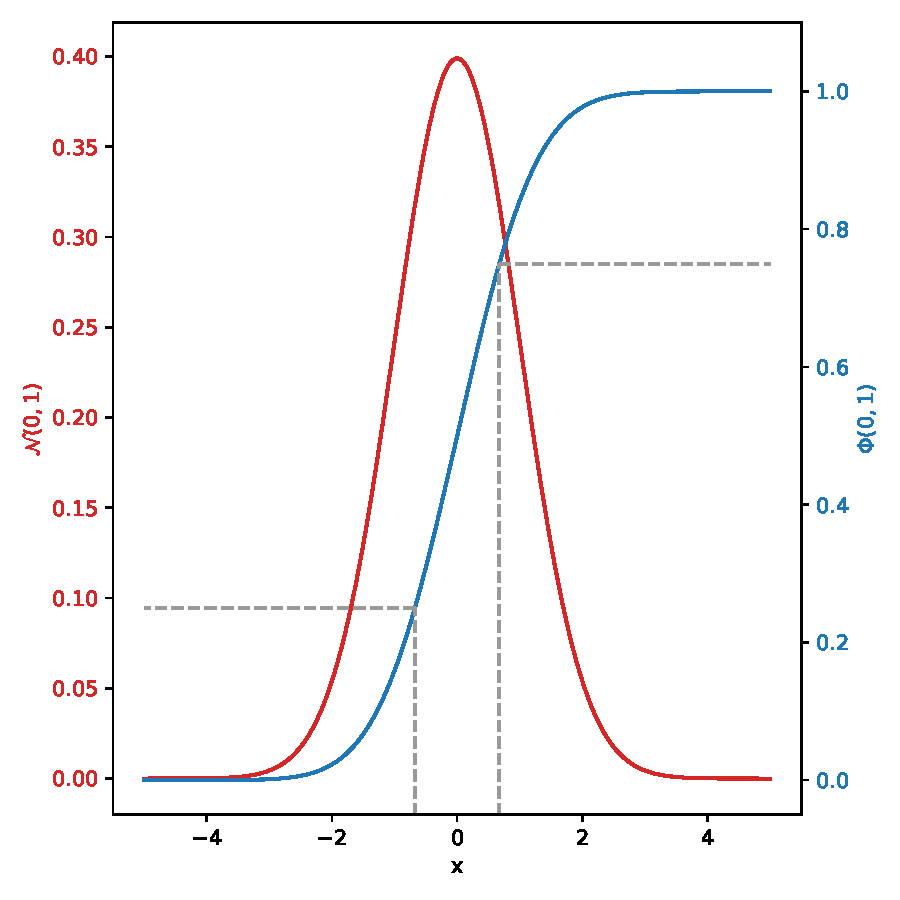
\includegraphics[width=0.7\textwidth]{phi.pdf}
\end{center}
\caption{Standard Gaussian distribution (red). Its cumulative distribution function (blue). First and last quartile indicated by grey dashed lines.}
\label{fig-cdf}
\end{figure}
  
  For any CDF $F$ that is monotonically increasing, there exists an inverse which is denoted by $F^{-1}$.  $F^{-1}(\alpha)$ is called
  the $\alpha$ \emph{quantile}. By definition, then, this is value $x_{\alpha}$ for which $P(X < x_{\alpha}) = \alpha$.
  The value of $F^{-1}(0.5)$ is called the \emph{median} of the distribution. The values of $F^{-1}(0.25)$ and $F^{-1}(0.75)$ are called
  the lower and upper \emph{quartiles}. They are shown in Fig \ref{fig-cdf}.

  The inverse CDF can be used to calculate \emph{tail area probabilities}. Points to the left of $F^{-1}(\alpha/2)$ contain $\alpha/2$
  of the probability mass. Points to the right of $F^{-1}(1 - \alpha /2)$ also contain $\alpha /2$ of the probability mass. The \emph{central interval}
  $(F^{-1}(\alpha/2), F^{-1}(1 - \alpha/2)$ contains $1 - \alpha$ of the probability mass. For example, for $\alpha = 0.05$, the 95 \% central interval
  is given by: $(\Phi^{-1}(0.025), \Phi^{-1}(0.975)) = (-1.96, 1.96)$.

  When $\mu, \sigma$ are accurately known, the $z$-score for a data point $x$ is given by $z=\frac{x-\mu}{\sigma}$. Using the $z$-score, a data point can be compared
  to the $\mathcal{N}(0,1)$ interval. For example, if a data point falls outside the central interval as calculated above, it is atypically large or small. 
  This is only possible when the parameters are accurately known rather than estimated. This is the case for very large populations, or comparing to ideal coins or dice
  and making predictions about the outcome using the central limit theorem.

  As an example, consider the height of UK males, which is given as 174.5 cm for the 50-percentile, 186.0 cm for the 95-percentile and 164.1 cm for the 5-percentile
  \cite{heights} (cited from \url{https://unece.org/fileadmin/DAM/trans/doc/2005/wp29grsp/HR-04-14e.pdf}).
  Assuming that
  the height distribution is a Gaussian and that these numbers were measured on a large sample of the population we find that apparently
  $\mu = 174.5$ and since $\Phi^{-1}(0.95) = 1.65$, this gives a $z$-score which we can find $\sigma$ by:
  $$
  \sigma = \frac{x_{95} - \mu}{z_{95}} = \frac{186.9 - 174.5}{1.65} = 7.52 \mbox{cm}
  $$
  We now have estimates for $\mu$ and $\sigma$ and should be able to make predictions about the 5-percentile, which we have not used in the calculation.
  $z_{05} = -1.65$ (as expected), giving $x_{05} = \mu + \sigma*z_{05} = 162.1$ cm which is in the right ball park, but shows a deviation from the reported value
  of 164.cm, suggesting heights are not distributed as a perfect Gaussian.

  The $z$-score is useful when the the Gaussian parameters are known, or when a score can be compared to a hypothetically perfect distribution like the Bernoulli
  distribution of a perfect coin. The average of $N$ observations will be Gaussian by the central limit theorem, so when we observe 100 coin tosses and calculate
  the $z$-score, we will be able to calculate the percentile function for this given outcome. We can then do a primitive form of hypothesis testing where the null hypothesis
  is that the coin is fair, and where we use an observation that has less than 5 \% probability under the assumption that the coin is fair to reject this hypothesis.

  When the parameters are not known, for example when the variance must be estimated from the data itself, the calculated $z-$score
  no longer follows a Gaussian distribution and other means like $t$-tests must be used. We will not discuss this further here. Standard statistic textbooks can
  be consulted, e.g. \cite{gardiner2009}.
  
\chapter{Multivariate Gaussian Distributions}

\begin{figure}[!ht]
\begin{center}
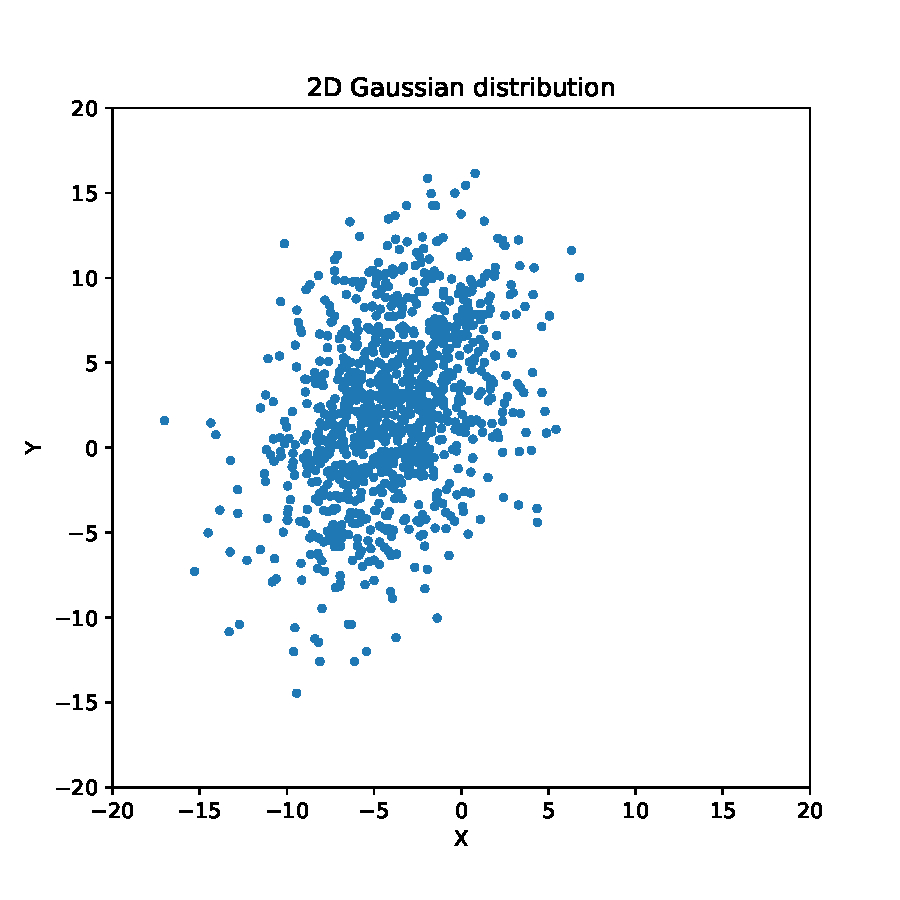
\includegraphics[width=0.7\textwidth]{gausssample.pdf}
\end{center}
\caption{Sample of a two dimensional Gaussian distribution in two variable: $X$ and $Y$. The variables are correlated and not centred at the origin.}
\label{fig-2dgauss}
\end{figure}
   \section{Introduction}

  Multivariate means that it is a distribution in more than one variable. An example of samples drawn from a two-dimensional distribution are shown in Fig. \ref{fig-2dgauss}.
  Before giving the formula for the multivariate Gaussian, a few remarks on notation.

  A data point in multivariate distribution of dimension $N$ is a tuple of $N$ numbers, which is usually represented as a vector. In much of the machine learning literature,
  vectors are indicated by boldface lower case symbols. E.g. suppose we record IQ and height of individuals we have a data points where one dimension is used to record
  the height of the individual and a second one to record the IQ. We denote the data point by:
  \begin{equation}
    {\bf x}_i = \left( \begin{array}{c} \mbox{iq}_i \\ \mbox{height}_i \end{array} \right)
  \end{equation}
  Some books use the vector notation $\vec{x}$, but the boldface notation is more prevalent.

  Mathematical purists might object that these data points are tuples rather than vectors and they would have a point, but many of the operations in machine learning rely
  on so-called matrix-vector manipulations by numerical software and it is easier to stick to the conventions used in the machine learning literature.

  The boldface notation indicates a column vector. Transposing it yields a row vector, so:
  \begin{equation}
    {\bf x}^T = ( \mbox{iq}, \mbox{height} )
  \end{equation}

  Matrix multiplication rules govern how expressions should be evaluated. If ${\bf v}$ and ${\bf w}$ are both $N$-dimensional vectors, then
  ${\bf v}^T {\bf w}$ represents the scalar product between these vectors, since it is the product of a row vector with a column vector, e.g.:
  $$
  \left( v_1, v_2 \right) \left( \begin{array}{c} w_1 \\ w_2 \end{array} \right) = v_1 w_1 + v_2 w_2. 
  $$
  On the other hand, $\boldsymbol{v} \boldsymbol{w}^T$ represents a matrix whose components are $v^iw_j$ as can be seen from:
  $$
  \left( \begin{array}{c} v_1 \\ v_2 \end{array} \right) \left( \begin{array}{cc} w_1 & w_2 \end{array} \right) =
  \left( \begin{array}{cc} v_1w_1 & v_1w_2 \\ v_2w_1 & v_2w_2 \end{array} \right)
  $$

  
  Matrices are indicated by boldface upper case symbols. Where matrix and vector dimensions match matrix vector multiplications are implied by the order in which
  symbols occur. So, ${\bf M} {\bf v}$,  represents a column vector:
  $$
  \sum^N_{j=1} M^i_j v^j,
  $$
 
  whereas ${\bf v}^T M {\bf w}$ represents a number:
  $$
  \sum_{i,j} v_i M^i_j w^j
  $$
  

  
  The boldface notation without component indices is usually more efficient and often unambiguous. Sometimes it is necessary to resort to components, in particular in proofs.

  The multivariate Gaussian distribution is given by:
  \begin{equation}
    \mathcal{N}(\boldsymbol{x} \mid  \boldsymbol{\mu}, \boldsymbol{\Sigma} ) = \frac{1}{(2 \pi)^{D/2}} \frac{1}{ \mid \mbox{det}(\boldsymbol{\Sigma}) \mid^{\frac{1}{2}} } \exp \left\{ -\frac{1}{2}(\boldsymbol{x} - \boldsymbol{\mu})^T  \boldsymbol{\Sigma}^{-1}   (\boldsymbol{x} - \boldsymbol{\mu}) \right\} 
  \end{equation}

  The functional dependence of the Gaussian on ${\bf x}$ is given by the \emph{Mahalanobis distance}:
  \begin{equation}
    \Delta^2 = (\boldsymbol{x} - \boldsymbol{\mu})^T \boldsymbol{\Sigma}^{-1}(\boldsymbol{x} - \boldsymbol{\mu})
  \end{equation}
  Here, $\boldsymbol{\mu}$ is an $M$-dimensional vector, and $\boldsymbol{\Sigma}$ an $M \times M$ matrix. Without loss of generality, we can assume that $\boldsymbol{\Sigma}$ is a symmetric matrix.

  Any matrix $\boldsymbol{M}$ can be written as the sum of a symmetric and an anti-symmetric matrix:
  $$
  \boldsymbol{M}^i_j = \frac{1}{2}(\boldsymbol{M}^i_j + M^j_i) + \frac{1}{2}(\boldsymbol{M}^i_j - M^j_i)
  $$
  You should verify that the anti-symmetric part does not contribution to the term under exponential, so we can always assume that $\boldsymbol{\Sigma}$ is symmetric.

  
  
  \subsection{Spectral Decomposition of the Covariance Matrix}
  \emph{The material in this section is relatively abstract. A Jupyter notebook titled: {\bf Eigenvectors of the Covariance Matrix} contains
    a worked example of the concepts discussed in this section.}
  
  It is well known from linear algebra that a symmetric matrix can be diagonalised if a coordinate transformation is carried out from the original
  coordinate system wherein the data points are represented to an orthonormal basis comprised of the eignvectors of the matrix.

  
  The eigenvector equation
  for the covariance matrix is:
  $$
  \boldsymbol{\Sigma}\boldsymbol{u}_i = \lambda_i \boldsymbol{u}_i,
  $$
  where $i = 1, \cdots, D$.

  In practice, in machine learning, we will find both eigenvectors and eigenvalues using numerical method. The notebook \emph{Eigenvectors of the Covariance Matrix}
  gives examples and shows how the concepts discussed below apply to the Gaussian distribution.
  In general, any symmetric $D \times D$ matrix has $D$ real eigenvalues. Moreover, the eigenvectors corresponding to these eigenvalues can be chosen to be orthonormal, i.e.
  \begin{equation}
    \boldsymbol{u}^T_i\boldsymbol{u}_j = \mathbb{1},
  \end{equation}
  where $\mathbb{1}$ is the $D$-dimensional identity matrix.
  The matrix $\boldsymbol{U}$ is a matrix where row $i$ is given by $\boldsymbol{u}^T_i$

  Now introduce:  
  $$
  \boldsymbol{y}_i = \boldsymbol{u}^T_i(\boldsymbol{x} - \boldsymbol{\mu})
  $$
  The $\boldsymbol{y}_i$ are new coordinates which are translated and rotated with respect to the old ones. Forming the vector
  $\boldsymbol{y} = (\boldsymbol{y}_1, \cdots, \boldsymbol{y}_D$, one can write:
  $$
  \boldsymbol{y} = \boldsymbol{U}(\boldsymbol{x} - \boldsymbol{\mu} )
  $$

  What this achieves is that, first the distribution is centred at the origin, and then a rotation is to the distribution so that the coordinate axes
  coincide with the eigenvectors (this is possible because the eigenvectors are orthonormal, so a rotation exists that aligns the eigenvectors
  with the coordinate axes; the rotation matrix is given by $\boldsymbol{U}$).

  In the new coordinate system the distribution is the product of $D$ independent Gaussian distributions:
  \begin{equation}
    p(\boldsymbol{y}) = \Pi^D_{j=1} \frac{1}{(2 \pi \lambda_j)^{1/2}} \exp \left\{-\frac{y^2_j}{2 \lambda_j} \right\}
  \end{equation}

  If you are familiar with the process of diagonalising a matrix, this is what we have just done. We have diagonalised
  $\boldsymbol{\Sigma}$ to the diagonal matrix $\mbox{diag}(\lambda_1, \cdots, \lambda_D)$.  For a diagonalised matrix the distribution factorises.
  
  
 
  
%\item A coordinate transformation  transforming the original basis to the basis of eigenvectors can be represented
%    by an orthonormal matrix $\boldsymbol{U}$, i.e. a matrix for which $\boldsymbol{U}^T\boldsymbol{U} = \boldsymbol{U} \boldsymbol{U}^T =  \mathbb{1}$.
%  \item The matrix $\boldface{\Sigma}$ is diagonalised by the transformation $\boldsymbol{U}^{-1} \boldsymbol{\Sigma} \boldsymbol{U}$.
%  end{enumerate}


  
  It is sometimes convenient to build a covariance matrix from a set of eigenvectors and eigenvalues.
  The spectral decomposition theorem states that covariance matrix can be expressed as an expansion in terms of its eigenvectors:
  \begin{equation}
    \boldsymbol{\Sigma}=\sum_{i=1}^{D} \lambda_{i} \mathbf{u}_{i} \mathbf{u}_{i}^{\mathrm{T}}
    \label{eq-spect}
  \end{equation}
  For the inverse:
    \begin{equation}
      \boldsymbol{\Sigma}^{-1}=\sum_{i=1}^{D} \frac{1}{\lambda_{i}} \mathbf{u}_{i} \mathbf{u}_{i}^{\mathrm{T}}
      \label{eq-spectinverse}
  \end{equation}

  
  This has useful applications. In \emph{Activity The Central Limit Theorem} you will learn how you can employ this equation to generate synthetic data sets.

  
  
  
  
  \subsection{Maximum Likelihood Estimation}
  We will derive the maximum likelihood estimators for $\boldsymbol{\mu}$ and $\boldsymbol{\Sigma}$. It is more important that you are able to read the resulting formulae and can
  convert them into working code than that you can perform these derivations. We will not assess  you on them. Having said that, if you want to be able to engage with the
  theoretical literature in the future you should be able to follow the derivations below and if not, you should acquire the matrix algebra underlying them.
  Appendix C of \cite{bishop2006} provides a relatively comprehensive summary of the results.
  If you do not want to follow the details of the derivation, skip until Eqs. \ref{eq-multivarMLE1} and \ref{eq-multivarMLE2}.
  
  Given a set of data points, that we suspect are Gaussian, how do we determine its parameters? Assume that we have a data set $\boldsymbol{X} = (\boldsymbol{x}_1, \cdots, \boldsymbol{x}_N)^T$.
  Note that this is a matrix with each individual data point constituting one row of the matrix. For $N$ data points, each of dimension $D$,
  the log likelihood function is given
  by:
  \begin{equation}
    \ln p(\boldsymbol{X} \mid \boldsymbol{\mu, \Sigma}) = -\frac{ND}{2} \ln (2\pi) - \frac{N}{2} \ln \mbox{det}(\boldsymbol{\Sigma}) -\frac{1}{2} \sum^N_{n=1}(\boldsymbol{x}_n - \boldsymbol{\mu})^T
        \boldsymbol{\Sigma}^{-1}(\boldsymbol{x}_n - \boldsymbol{\mu})
      \label{eq-mlgauss}
  \end{equation}

  In the following we will use the following results from matrix algebra:
  The \emph{trace} of a matrix is the sum of its diagonal elements:
  \begin{equation}
    \mbox{Tr}{\boldsymbol{A}} = \sum^D_{i=1} A_{ii}
  \end{equation}

  For real symmetric matrices, remember that they can be diagonalised by means of a rotation:
  \begin{equation}
    \boldsymbol{A} = \boldsymbol{U} \boldsymbol{\Lambda} \boldsymbol{U}^T,
    \label{eq-diag}
  \end{equation}
  where $\Lambda = \mbox{diag}(\lambda_1, \cdots, \lambda_D)$, the diagonal matrix with the eigenvalues of $\boldsymbol{A}$ at the
  diagonal entries.

  It can be shown that this has as consequence that
  \begin{equation}
    \mbox{det}(\boldsymbol{A}) = \Pi^D_{i=1} \lambda_i,
    \label{eq-producteig}
  \end{equation}
  and
  \begin{equation}
    \mbox{Tr}(\boldsymbol{A}) = \sum^D_{i=1} \lambda_i
  \end{equation}
  Both these results depend on Eq. \ref{eq-diag} so hold for real symmetric matrices, but not in general.

  The following results from matrix algebra can be proven simply by writing them out in components:
  \begin{align}
    \frac{\partial }{\partial  \boldsymbol{a}}\boldsymbol{b}^T \boldsymbol{a} & = \boldsymbol{b}  \\
    \frac{\partial}{\partial \boldsymbol{a}}(\boldsymbol{a}^T \boldsymbol{A} \boldsymbol{a}) &  = (\boldsymbol{A} + \boldsymbol{A}^T)\boldsymbol{a} \label{eq-tp} \\
    \frac{\partial}{\partial \boldsymbol{A}}\mbox{Tr}(\boldsymbol{B} \boldsymbol{A}) & = \boldsymbol{B}^T   \\
  \end{align}
  also easy to verify is:
  \begin{equation}
    \mbox{Tr}(\boldsymbol{A} \boldsymbol{B} \boldsymbol{C}) =     \mbox{Tr}(\boldsymbol{C} \boldsymbol{A} \boldsymbol{B}) =     \mbox{Tr}(\boldsymbol{B} \boldsymbol{C} \boldsymbol{A}) 
    \end{equation}
   
    
    With the last rule it is easy to justify the so-called \emph{trace trick}:
    \begin{equation}
      \boldsymbol{x}^T \boldsymbol{A} \boldsymbol{x} = \mbox{Tr}( \boldsymbol{x}^T \boldsymbol{A} \boldsymbol{x} ) = \mbox{Tr}( \boldsymbol{x} \boldsymbol{x}^T \boldsymbol{A} ) =\mbox{Tr}( \boldsymbol{A} \boldsymbol{x} \boldsymbol{x}^T )
    \end{equation}

    If the first equality baffles you, remember that the first term is a row vector, left multiplying a matrix, left multiplying a column vector. But a column row can also
    be interpreted as an $1 \times N$ matrix, and a column vector as an $N \times 1$ vector, so this a product of three matrices.

    Based on the spectral decomposition Eq. \ref{eq-spect}, \ref{eq-spectinverse}, and Eq. \ref{eq-producteig} as well as $\boldsymbol{u}^T_i \boldsymbol{u}_j  = I$ one can show:
    $$
      \frac{\partial}{\partial x} \ln \mbox{det}(\boldsymbol{A}) = \mbox{Tr} \left( \boldsymbol{A}^{-1}   \frac{\partial \boldsymbol{A}}{\partial x} \right),
    $$
    which specialises to:
    \begin{equation}
      \frac{\partial}{\partial \boldsymbol{A}} \ln \mbox{det}(\boldsymbol{A}) = ( \boldsymbol{A}^{-1})^T = \boldsymbol{A}^{-T},
    \end{equation}
    where the last equality introduces a convenient shorthand for the transpose of the inverse of a matrix.

    
  To estimate $\mu_{ML}$ we set:
  $$
  \frac{\partial}{\partial \boldsymbol{\mu} }\ln p(\boldsymbol{X} \mid \boldsymbol{\mu, \Sigma}) \mid_{\mu = \mu_{ML}} = 0
  $$
  
  Only terms that depend on $\boldsymbol{\mu}$ in Eq. \ref{eq-mlgauss}  are relevant:
  $$
  \frac{\partial}{\partial \boldsymbol{\mu}} \sum^N_{i=1}(\boldsymbol{x}_i - \boldsymbol{\mu})^T \boldsymbol{\Sigma}^{-1} (\boldsymbol{x}_i - \boldsymbol{\mu}) \mid_{\mu = \mu_{ML}} = 0
  $$

  By virtue of identity \ref{eq-tp} this is equivalent to:
  $$
   -\sum^N_{i=1} (\boldsymbol{\Sigma}^{-1} + {\boldsymbol{\Sigma}^{-T}})(\boldsymbol{x}_i - \boldsymbol{\mu}) \mid_{\mu = \mu_{ML}} = 0,
  $$
   From this it follows that
   $$
   -2 \boldsymbol{\Sigma}^{-1}( \sum^N_{i=1} x_i - N \boldsymbol{\mu}) \mid_{\mu = \mu_{ML}} = 0
   $$
   since $\boldsymbol{\Sigma} = \boldsymbol{\Sigma}^T$, and therefore:
   \begin{equation}
     \boldsymbol{\mu}_{ML} = \frac{1}{N} \sum^N_{i=1} {\bf x}_i
     \label{eq-multivarMLE1}
   \end{equation}
   The MLE of $\mu$ is the \emph{empirical mean}.

   To produce an MLE of the covariance matrix, it is convenient to introduce the \emph{precision matrix}, which is the inverse of
   the covariance matrix:
   \begin{equation}
     \boldsymbol{\Lambda} = \boldsymbol{\Sigma}^{-1}
   \end{equation}

   The only terms in the log likelihood that involve the covariance matrix
   are:
   $$
   \mathcal{L} = - \frac{N}{2} \ln \mbox{det}(\boldsymbol{\Sigma}) - \frac{1}{2} \sum^N_{i=1}(\boldsymbol{x}_i - \mu)^T \boldsymbol{\Sigma}^{-1}(\boldsymbol{x}_i - \boldsymbol{\mu})
   $$
   Expressed in terms of the precision matrix $\Lambda$ this reads:
   \begin{equation}
   \mathcal{L}(\boldsymbol{\Lambda}) = \frac{N}{2} \ln \mbox{det}(\boldsymbol{\Lambda}) - \frac{1}{2}  \sum^N_{i=1}(\boldsymbol{x}_i - \mu)^T \boldsymbol{\Lambda}(\boldsymbol{x}_i - \boldsymbol{\mu})
   \end{equation}
   where we used $\mbox{det}(\boldsymbol{\Lambda}) \mbox{det}(\boldsymbol{\Sigma}) = 1$, which follows from:
   $$
   \mbox{det}(\boldsymbol{AB}) = \mbox{det}(\boldsymbol{A})\mbox{det}(\boldsymbol{B})
   $$
   Employing the trace trick on this expression gives:
   \begin{align}
     \mathcal{L}(\boldsymbol{\Lambda}) & = \frac{N}{2} \ln \mbox{det}(\boldsymbol{\Lambda}) - \frac{1}{2}  \sum^N_{i=1}\mbox{Tr}(\boldsymbol{x}_i - \boldsymbol{\mu})^T \boldsymbol{\Lambda}(\boldsymbol{x}_i - \boldsymbol{\mu}),\nonumber \\
                          & = \frac{N}{2} \ln \mbox{det}(\boldsymbol{\Lambda}) - \frac{1}{2} \mbox{Tr}(\boldsymbol{S}_{\mu} \boldsymbol{\Lambda}),
   \end{align}
   where the scatter matrix
   \begin{equation}
     \boldsymbol{S}_{\mu} \equiv  \sum^N_{i=1}({\bf x}_i - {\boldsymbol{\mu}})({\bf x}_i - \boldsymbol{\mu})^T
   \end{equation}

   The MLE for the precision matrix is very easy to derive in this form:
   $$
   \frac{\partial \mathcal{L}(\boldsymbol{\Lambda})}{\partial \boldsymbol{\Lambda}} \mid_{\Lambda = \Lambda_{ML}} = \frac{N}{2} \boldsymbol{\Lambda}^{-T} -
   \frac{1}{2}\boldsymbol{S}^T_{\mu} = 0. 
   $$
   Using $\boldsymbol{\Lambda}^{-T} = \boldsymbol{\Lambda}^{-1} = \boldsymbol{\Sigma}$, we find:
   \begin{equation}
     \boldsymbol{\Sigma}_{ML} = \frac{1}{N}\boldsymbol{S}_{\mu} = \frac{1}{N}\sum^N_{i=1}(\boldsymbol{x}_i - \boldsymbol{\mu})(\boldsymbol{x}_i - \boldsymbol{\mu})^T
     \label{eq-multivarMLE2}
   \end{equation}
    
   \section{Completing the Square - Marginal and Conditional Probabilities of the Gaussian}
   In general, when given a high dimensional distribution it is difficult to marginalise
   with respect to given variables because this entails integration in high dimensional
   spaces unless one is fortunate enough to be able to integrate analytically. Normalising
   a distribution can be difficult for the same reason.

   Gaussian distributions allow analytic integration and thereby marginalisation and normalisation. The technique occurs often enough
   in the machine learning literature to  warrant an activity centred around this topic.
   A simple but important observation is that the log likelihood of a Gaussian is a quadratic form. Usually, it is sufficient to manipulate
   this quadratic form and restore the original distribution after the fact.

   To see this, observe that:
   \begin{equation}
   -\frac{1}{2} (\boldsymbol{x} - \boldsymbol{\mu})^T \boldsymbol{\Sigma}^{-1} ( \boldsymbol{x} - \boldsymbol{\mu}) =
   -\frac{1}{2}\boldsymbol{x}^T \boldsymbol{\Sigma}^{-1} + \boldsymbol{x}^T \boldsymbol{\Sigma}^{-1} \boldsymbol{\mu} + \mbox{const}
   \end{equation}
   When the log likelihood is brought into the form of the lefthand side, the full distribution is easily restored: it just requires exponentiating the quadratic
   form, and obtaining the overall normalisation factor which a function of the covariance matrix $\Sigma$ only. When the log likelihood is in the form
   of the righthand side, it can be brought into the form of the lefthand side by completing the square.

   In practice, this means that if the linear and quadratic terms of the log likelihood
   are known, the entire probability distribution can be reconstructed. Many
   mathematical operations involving Gaussians can be performed by  manipulating
   quadratic forms. If this is not clear now, in Activity \emph{Completing the Square: Manipulating the Gaussian log likelihood },
   we will also show that if prior and likelihood are
   Gaussian, the posterior is Gaussian again, a fact that can be used immediately in
   Bayesian Linear Regression.
  %%
   % The back matter contains appendices, bibliographies, indices, glossaries, etc.
  
\chapter{Bayesian Linear Regression}

\section{Introduction}

\begin{figure}
\begin{center}
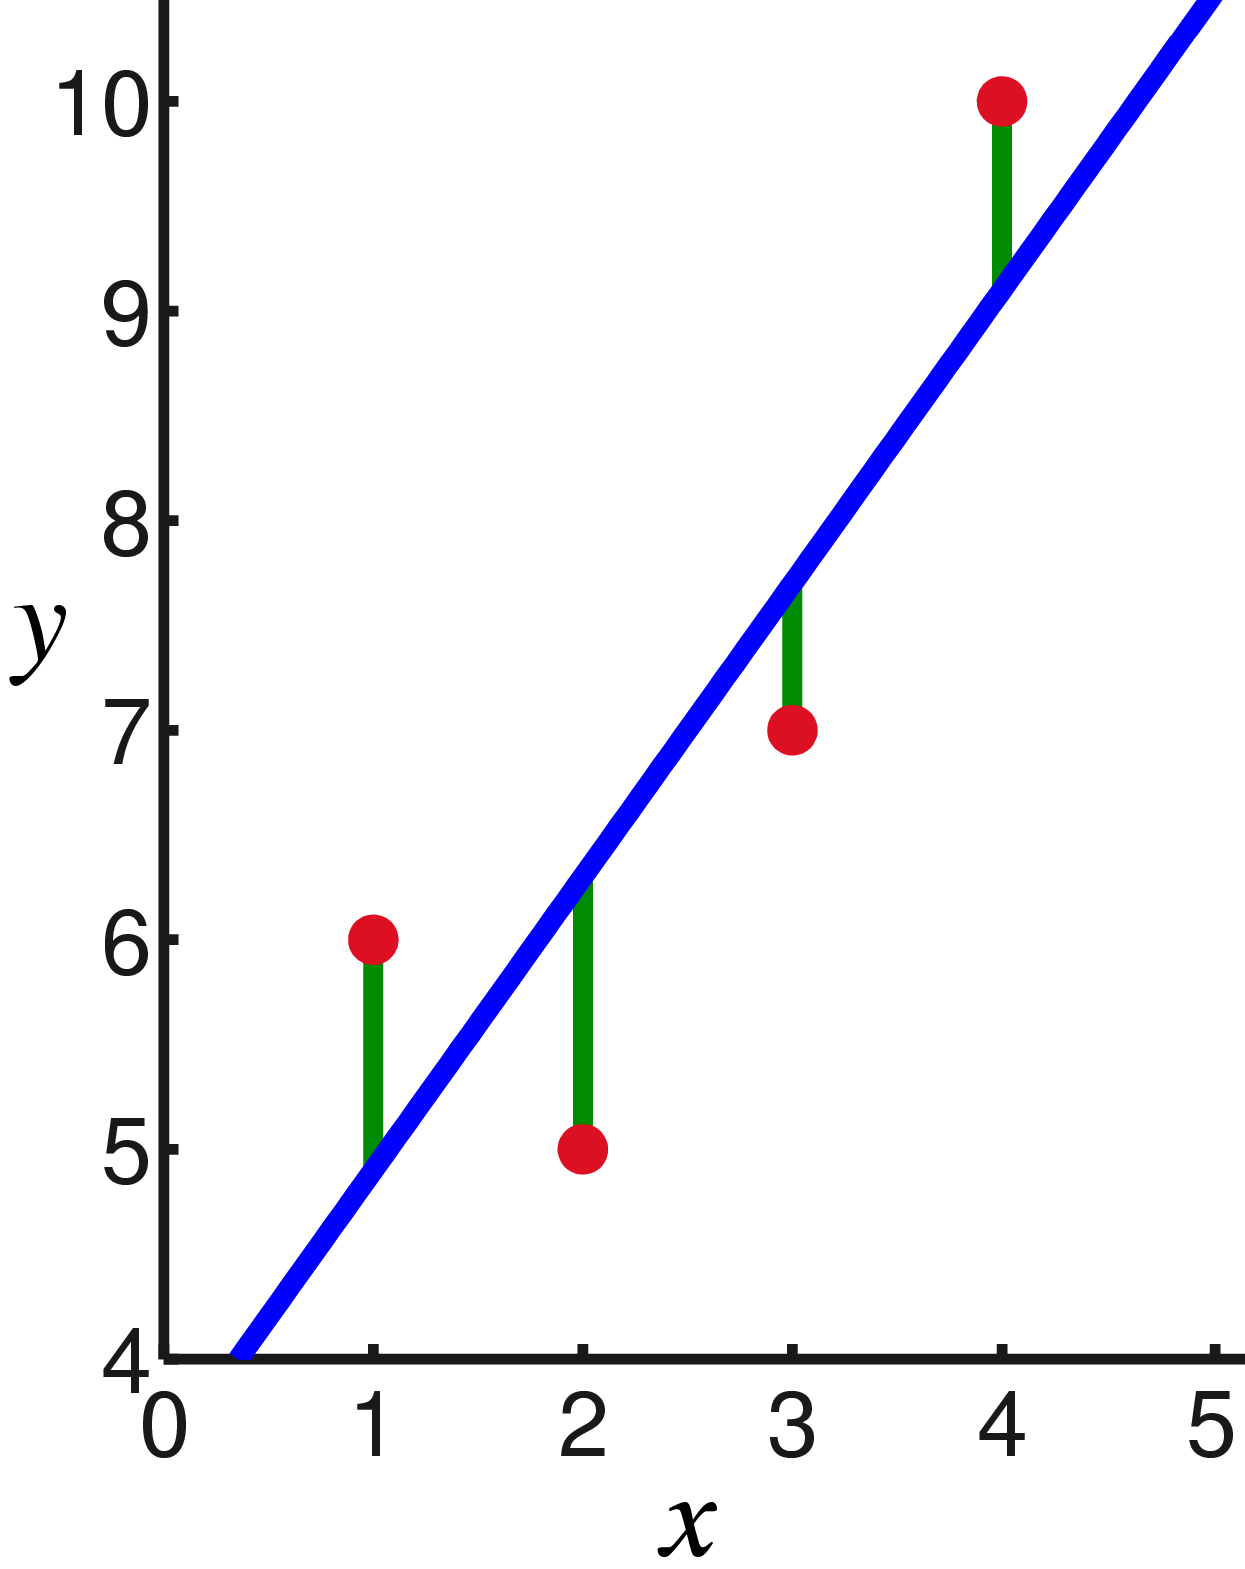
\includegraphics[width=0.3\textwidth]{residu.png}
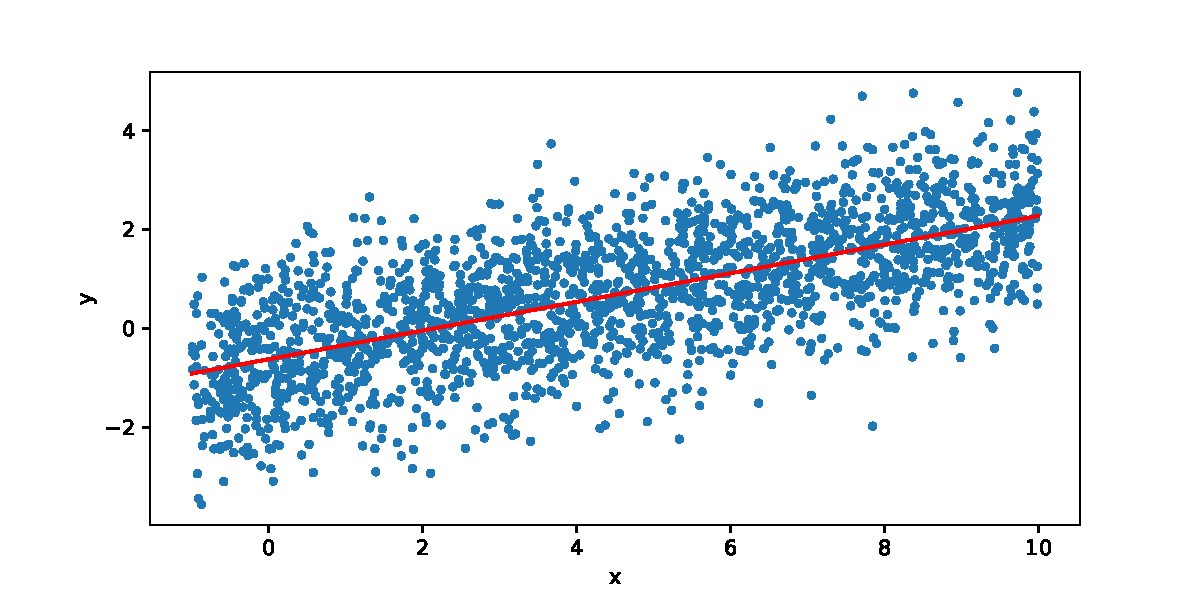
\includegraphics[width=0.65\textwidth]{linres.pdf}
\end{center}
\caption{Left: observed points in red. A line fit to these points in blue. The residues in green (Wikimedia-ccby). Right: An example of linear regression.}
\label{fig-linres}
\end{figure}

The purpose of this section is to introduce the algebraic structure of linear regression, to contrast it in the next section with Bayesian linear regression. It
is not necessary to be able to perform the  derivations yourself, but you should be able to apply the resulting formulae. Examples of such applications are given
in the notebook \emph{Example 1.7: Linear Regression}.


   The technique of linear regression is widely used in statistics and machine learning. You are expected to be familiar with it, because it was presented in the
   Data Science module. The essence of the method is shown in Fig. \ref{fig-linres}, where a linear functional relationship between
   two variables $x$ and $y$ is assumed, but where this relationship is imperfect, for example due to noise. It is clear that no linear relationship can fit the data
   perfectly, but on the other hand representation of the data by a linear function has a number of advantages. First, it requires much less information to store
   the parameters of the line than the entire data set. The linear function is called a \emph{regression function} and the data is said to be regressed to a linear
   relationship. Second, the linear function may be used for \emph{prediction}: when a new value of $x$ is presented, the
   linear relation should present a reasonable prediction of $y$.

   It is clear that some lines will be a good fit, and the line shown in Fig. \ref{fig-linres} is the best line in the following sense. It is clear  that none
   of the data points are perfectly represented by the line. Consider a data point $(x_i, y_i)$ and a model line $y = ax + b$ with $a, b$ known parameters.
   For a given data point $r_i = y_i -(ax_i + b)$, the residue of point $i$ represents a mismatch between the model prediction for value $x_i$, $ax_i + b$, and its actual
   value, $y_i$. Consider the sum of all residues squared: $R = \sum_i r^2_i$. For unknown $a, b$,$R$ can be considered a function of $a$ and $b$. OLS finds the values
   of $a, b$ that minimise this function. Since $R$ is essentially a quadratic function in $a$ and $b$, we can be assured that a single global minimum exists. This
   should be expected, if we shuffle the line around in Fig. \ref{fig-linres}, it is clear that some sort of optimum line can be found.

   
   Algebraically, conditions values for $a$ and $b$ can be found by minimising the function:
   $$
   R = \sum^N_{i=1} (y_i -(ax_i + b))^2,
   $$
   where $N$ is the number of data points.
   
   Differentiation with respect to $a$ and $b$ and setting the derivatives to 0 gives conditions for find the minimum:
   \begin{align}
     \frac{\partial}{\partial a}R(a, b) &  = 0 \nonumber \\
     \frac{\partial}{\partial b}R(a,b)  &  = 0 \nonumber
   \end{align}


   This works out as a linear system of two equations with two unknowns:
   \begin{align}
     \sum_i x_iy_i & = a \sum_i x^2_i + b \sum_i x_i \nonumber \\
     \sum_i y_i    & = a \sum_i x_i   + bN
   \end{align}

   
   
   In this particular case, formulae for $a$ and $b$ can easily be found by solving this system, which are the famous linear regression formulae.

   A formal solution can be found by writing it in matrix-vector form:
   \begin{equation}
     \left( \begin{array}{c} a \\ b \end{array} \right) = \left( \begin{array}{cc} \sum_i  x^2_i &  \sum_i x_i \\ \sum_i x_i & N \end{array} \right)^{-1}
     \left( \begin{array}{c} \sum_i x_iy_i \\ \sum_i y_i \end{array} \right)
   \end{equation}

   
   It is perfectly possible to include higher order terms, and for example fit a second
   degree polynomial to the data. A second degree polynomial has three parameters
   and would lead three equations with three unknowns that can solved directly. We
   will formulate this approach in way that allows easy generalisation to arbitrary
   degree.

   Introduce the vector $\phi(x_i)$, defined as:

   \begin{equation}
     \phi(x_i) = \left( \begin{array}{c} 1 \\ x_i \\ x^2_i \end{array} \right)
   \end{equation}

   and a vector $\boldsymbol{w}$:
   \begin{equation}
     \boldsymbol{w} = \left( \begin{array}{c} w_0 \\ w_1 \\ w_2 \end{array} \right),
   \end{equation}
   so that:
   $$
   \boldsymbol{w}^T \boldsymbol{\phi}(x)= w_0 + w_1x + w_2x^2
   $$
   indeed represents a general second degree polynomial. This idea
   easily generates to a polynomial of arbitrary degree. If we are fitting
   an $M-1$ degree polynomial, we need $M$ parameters that we organise in an
   $M$-dimensional vector $\boldsymbol{w}$.

   The idea of minimising the residual squared sum is completely equivalent to
   that when regressing to a linear function:

   \begin{equation}
     R = \sum^N_{i=1} (y_i - \boldsymbol{w}^T \boldsymbol{\phi}(x_i))^2
     \label{eq-residuesq}
   \end{equation}

   Again, we will find the value for $\boldsymbol{w}_{OLS}$ by setting:
   $$
   \frac{\partial }{\partial \boldsymbol{w}} R \mid_{\boldsymbol{w} = \boldsymbol{w}_{OLS}} = 0
   $$

   Calculating the gradient leads to:
   $$
   \sum^N_{i=1} (t_i - \boldsymbol{w}^T \boldsymbol{\phi}( \boldsymbol{x}_i))
   \boldsymbol{\phi}(\boldsymbol{x}_i)^T = 0,
   $$
   or
   \begin{equation}
     \sum^N_{i=1} y_i \boldsymbol{\phi}^T(x_i)  = \boldsymbol{w}^T(\sum^N_{i=1} \boldsymbol{\phi}(x_i) \boldsymbol{\phi}^T(x_i))
     \label{eq-solodl}
   \end{equation}

   For each data point we have a column vector $\boldsymbol{\phi}(x_n)$. The \emph{design matrix} is an $N \times M$, matrix whose
   elements are given by $\Phi_{nj} = \phi_j(x_n)$.
   Here $M-1$ is the degree of the polynomial that we intend to fit to the data and $N$ is the number of data points. For the case
   of fitting a second degree polynomial, $M=3$.
   
\begin{equation}
\Phi = \left( \begin{array}{cccc} \phi_0(x_1) & \phi_1(x_1) & \cdots & \phi_{M-1}(x_1) \\
                                  \phi_0(x_2) & \phi_1(x_2) & \cdots & \phi_{M-1}(x_2) \\ 
                                  \vdots      & \vdots      &        & \vdots          \\
                                  \phi_0(x_N) & \phi_1(x_N) & \cdots & \phi_{M-1}(x_N) \end{array}\right)
\end{equation}

Using this matrix, we can write Eq. \ref{eq-solodl} as
$$
  \boldsymbol{\Phi}^T \boldsymbol{t}  = \boldsymbol{\Phi}^T\boldsymbol{\Phi} \boldsymbol{w},
  $$
  so that
  \begin{equation}
    \boldsymbol{w}_{OLS} = (\boldsymbol{\Phi}^T\boldsymbol{\Phi})^{-1} \boldsymbol{\Phi}^T\boldsymbol{t}
      \label{eq-moorepenrose}
  \end{equation}
  
  Some care must be used in applying these equations as they may be numerically unstable. This may happen
  if two basis functions evaluate to nearly the same vector. In that case an SVD decomposition must be used
  \cite{bishop2006}.
  

  Although Eq. \ref{eq-moorepenrose} is a very compact notation, the result is not
  fundamentally different from the linear regression example, nor is the reasoning leading
  to it. It is instructive to formulate the case of a straight line, which is a polynomial
  of degree 1, so $M=2$.

  The column vector for data point $x_i$ in this case is:
  $$
  \phi(x_i) = \left( \begin{array}{c} 1 \\ x_i \end{array} \right),
  $$
  so the design matrix $\Phi$ is given by:
  $$
  \Phi = \left( \begin{array}{cc} 1 & x_1 \\ 1 & x_2 \\ \vdots & \vdots \\ 1 & x_N \end{array} \right)
  $$
  so that its transpose $\Phi^T$ is:
   $$
  \Phi^T = \left( \begin{array}{cccc} 1 & 1 & \cdots & 1 \\ x_1 & x_2 & \cdots & x_N \end{array} \right),
  $$
  The product of the two is:
  \begin{equation}
    \Phi \Phi^T  = \left( \begin{array}{cc} N & \sum_i x_i \\ \sum_i x_i & \sum_i x^2_i \end{array} \right), 
   \end{equation}
  Since $\boldsymbol{t}$ is:
  $$
  \boldsymbol{t} = \left( \begin{array}{c} y_1 \\ y_2 \vdots \\y_N \end{array} \right),
  $$
  the formula for finding the appropriate coefficients (weights) for our polynomial is:
  \begin{equation}
    \left(  \begin{array}{c} w_0 \\ w_1 \end{array} \right)  =
    \left( \begin{array}{cc} N & \sum_i x_i \\ \sum_i x_i & \sum_i x^2_i \end{array} \right)^{-1} \left( \begin{array}{c} \sum_i y_i \\ \sum_i x_iy_i  \end{array} \right)
  \end{equation}

  
  Again, you will not be assessed on whether you can derive this result, but you are
  strongly encouraged to study notebook \emph{Example 1.7: Linear Regression}, to
  see how the design matrix is built from the data and how Eq. \ref{eq-moorepenrose}
  works out in practice.

\begin{figure}
\begin{center}
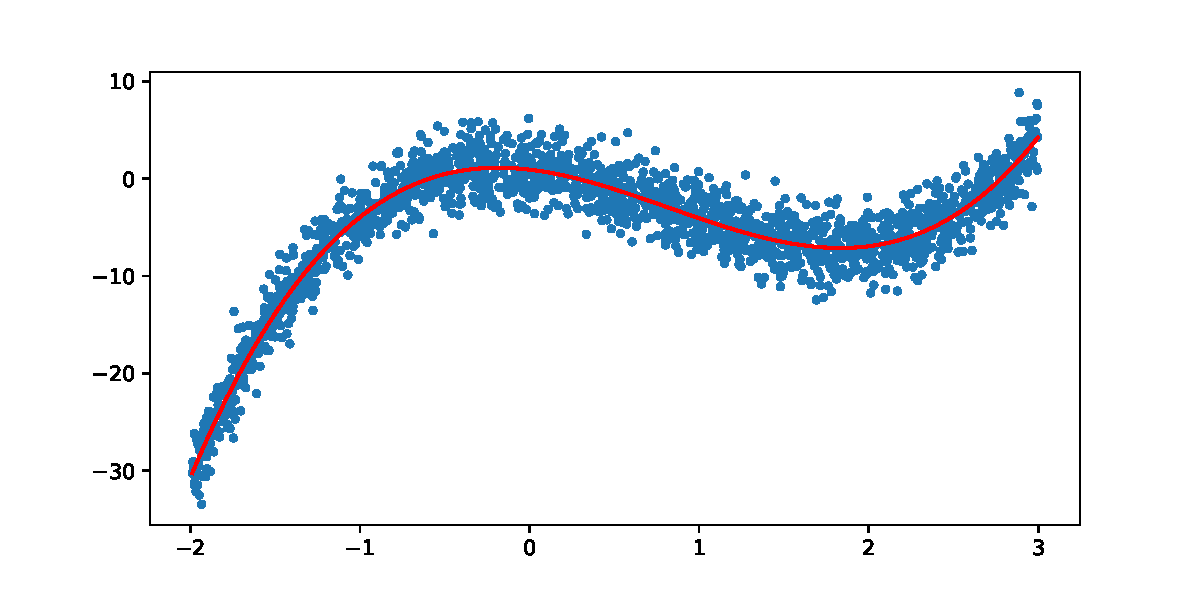
\includegraphics[width=0.7\textwidth]{cubic.pdf}
\end{center}
\caption{The result of linear regression on a cubic polynomial.}
\label{fig-cubic}
\end{figure}

Figure \ref{fig-cubic} shows the fit of a cubic
  
{\bf It is important to realise that all examples of this section are linear regression, even if we fit a non linear function to the data.} The distinction between
  linear and non linear regression is not  whether or not to use of linear functions to model the
  data, but whether the fit function is a linear function its weights. In that case
  Eq. \ref{eq-moorepenrose} applies.
  An example of non linear regression is \emph{logistic regression}, to be discussed in
  Unit 2.

  
  Also important is the realisation that polynomials are not the only function
  we can regress to. Any sufficiently rich set of \emph{basis functions} can
  be used. In the case of fitting to a polynomial, the basis functions are
  the \emph{monomials} $1, x, x^2, \cdots$. But Gaussians can also be used as basis
  functions. For example, if functions in a range $[a,b]$ need to be modeled, one
  can create a grid in $\mu, \sigma$ representing Gaussians of different means
  and variances. The notebook \emph{Example 1.7: Linear Regression} gives a simple
  example of that.

  So, the vector of functions $\boldsymbol{\phi}(x)$ can be chosen differently,
  but the process of constructing the design matrix and the regression procedure remain
  the same, given $\boldsymbol{\phi}(x)$, which are sometimes called \emph{features}.
  For this reason linear regression is a powerful framework that is applicable to
  data with very non linear features. 


\begin{figure}[!ht]
\begin{center}
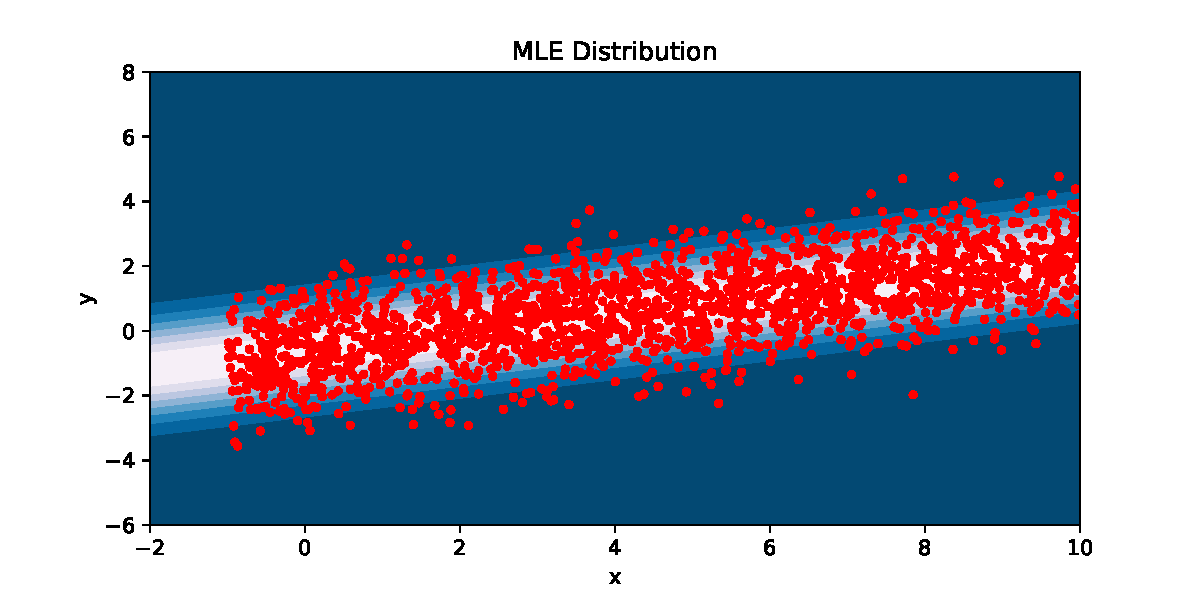
\includegraphics[width=0.7\textwidth]{mle.pdf}
\end{center}
\caption{The MLE, a single point in $(\mu, \sigma)$ space, determines a Gaussian distribution centred around the line represented by the MLE.}
\end{figure}  

  

  \section{Maximum Likelihood and Least Squares}
  In the ordinary least squares approach from the previous section no particular assumption was made about the origin of the residuals. Here we will see
  that it has a natural interpretation as the maximum likelihood estimation of a deterministic model with additive Gaussian noise.

  Assume that we are observing data that has been generated by a process that can be described by
  \begin{equation}
    t = y (\boldsymbol{x}, \boldsymbol{w}) + \epsilon,
    \label{eq-noise}
  \end{equation}
  where $\epsilon$ is a Gaussian variable with zero mean and \emph{precision} $\beta$ (precision is the inverse of variance so $\beta = 1/\sigma$, its use is a matter of convenience, unburdening the notation of $^{-1}$s).
    In general, we will know the function $y$, but not the parameters $\boldsymbol{w}$, which we will  have to infer from the observed data, just as in the case of
    linear regression.  

    Eq. \ref{eq-noise} implies the existence of a probability distribution of target values, condition $\boldsymbol{x}$ and parameters $\boldsymbol{w}$
    through the deterministic function $y$:
    \begin{equation}
      p(t \mid \boldsymbol{x}, \boldsymbol{w}, \beta) = \mathcal{N}(t \mid y(\boldsymbol{x}, \boldsymbol{w}), \beta^{-1} )
        \label{eq-noisedet}
    \end{equation}

    Consider the data set of inputs $\boldsymbol{X} = \left\{ \boldsymbol{x}_1, \cdots, \boldsymbol{x}_N \right\}$ with corresponding target values $t_1, \cdots t_N$,
    we group the targets values $\left\{ t_i \right \}$ into a column vector $\boldsymbol{t}$. Assuming data points are independently drawn from distribution
    \ref{eq-noisedet}, it is possible to define a likelihood function with adjustable parameters $\boldsymbol{w}$ and $\beta$
    \begin{equation}
      p(\boldsymbol{t} \mid \boldsymbol{X}, \boldsymbol{w}, \beta) = \Pi^{N}_{i=1} \mathcal{N}(t_i \mid \boldsymbol{w}^T \boldsymbol{\phi}(\boldsymbol{x}_i), \beta^{-1}),
      \label{eq-gaussllh}
    \end{equation}
    where, as usual, $\mathcal{N}$ denotes the Gaussian distribution.
    The log likelihood then is:
    \begin{align}
      \ln p(\boldsymbol{t} \mid \boldsymbol{w}, \beta ) & = \sum^N_{i=1} \ln \mathcal{N}(t_i \mid \boldsymbol{w}^T \boldsymbol{\phi}(\boldsymbol{x}_i),\beta^{-1}) \nonumber \\
      & = \frac{N}{2} \ln \beta - \frac{N}{2} \ln ( 2 \pi ) - \beta E_{D}(\boldsymbol{w})
    \end{align}
    Here, the sum-of-squares error function is given by:
    \begin{equation}
      E_D(\boldsymbol{w}) = \frac{1}{2} \sum^N_{i=1}(t_i - \boldsymbol{w}^T \boldsymbol{\phi}(\boldsymbol{x}_i))^2
    \end{equation}
    But this is the same form as the sum of squared residues Eq. \ref{eq-residuesq}! So, the estimate for $\boldsymbol{w}$ that minimises the log likelihood and thereby
    maximises the likelihood, $\boldsymbol{w}_{MLE}$ is the same that minimises the
    sum of residues squared, and we find:

  \begin{equation}
    \boldsymbol{w}_{MLE} = (\boldsymbol{\Phi}^T\boldsymbol{\Phi})^{-1} \boldsymbol{\Phi}^T\boldsymbol{t}
      \label{eq-moorepenrose2}
  \end{equation}
    
  It is important to note that no particular noise model underlies the OLS estimates,
  whereas the interpretation of $\boldsymbol{w}_{MLE}$ as maximum likelihood estimate
  explicitly determines on the Gaussian assumption made in Eq. \ref{eq-noisedet}.
  However, when the Gaussian model is appropriate it allows a more extensive analysis
  for example Bayesian linear regression.




  
  \section{Bayesian Linear Regression}
  Bayesian linear regression is a vast subject, and here we only give a bare bones introduction. The key idea is the same as in our example
  of the false coin: we assume that our parameters are uncertain and model this with a probability distribution. You are forced to assume
  a prior distribution, but as data becomes available, you use it to infer a posterior distribution \emph{given} the data. This distribution
  will become more and more focused as more data becomes available. In the limit of infinite data, the distribution would become a sharp
  narrow peak that centres a value. In this limit the maximum likelihood would also converge on this value and both approaches would give
  the same result: a specific numerical prediction that contains no uncertainty. When not much data is available, the posterior distribution
  will be wider, representing the uncertainty in our fit parameters. MLE on the other hand will produce point estimate for them. Only with cross
  validation do we get a feeling for the uncertainty in this estimate.

  The Bayesian linear regression case is  an important illustration of the fact that:
  \emph{Bayesian  methods are less prone to overfitting than MLE estimates}. The concept of regularisation emerges as a natural consequence
  of the Bayesian approach, and Bayesian linear regression serves as a good demonstration.


    As in the earlier example of the false coin where we had to assume a prior distribution for the parameter $\mu$, we define a prior distribution
  for the weights $\boldsymbol{w}$:
  \begin{equation}
    p(\boldsymbol{w}) = \mathcal{N}( \boldsymbol{m}_0, \boldsymbol{S}_0 )
  \end{equation}

  The likelihood function is given by:
  \begin{equation}
    \mathcal{L} = \Pi^N_{i=1} \mathcal{N}(t_i \mid \boldsymbol{w}^T \boldsymbol{\phi}(x_i), \beta^{-1}),
  \end{equation}
  which is the same we used in the case of the MLE.
  
  Throughout this example, we will assume that $\beta$, the precision, is known. If it is not known, the approach can be extended
  to infer it as well, although  there will be some technical difficulties that we do not want to address here. Here we will
  use the data to infer the set of weights $\boldsymbol{w}$ that will describe the data best.

  In this particular case Bayes' rule can be written as:
  \begin{equation}
    p(\boldsymbol{w} \mid \boldsymbol{X}, \boldsymbol{t}, \alpha, \beta) \sim
    p(\boldsymbol{t} \mid \boldsymbol{X} \boldsymbol{w} \beta) p (\boldsymbol{w} \mid \alpha)
  \end{equation}

  
  
  It is a relatively straightforward exercise, which you will do yourself in a worksheet, to show
  that for a Gaussian prior the posterior will also be a Gaussian. In this exercise you will
  find the mean and covariance of the posterior distribution in terms of the data
  and the mean and covariance of the prior distribution. 


Here, we briefly state the formulae for Bayesian Linear regression. 
Again we want to describe our data with a deterministic polynomial, whose coefficients we want to determine from the data. In line with the
Bayesian approach, we define a prior probability distribution over our weights. Based on the assumption of Gaussian distributed noise \ref{eq-gaussllh}, we assume a Gaussian
prior:
$$
p(\boldsymbol{w}) = \mathcal{N}(\boldsymbol{w} \mid 0, \alpha^{-1}\mathbb{1}),
$$
that is: we centre our weights on zero and allow a single parameter to set the variance in each dimension.
In the absence of prior knowledge about the data, this is a reasonable choice.

The posterior distribution is Gaussian again:
$$
p(\boldsymbol{w} \mid \mathcal{D} ) = \mathcal{N}(\boldsymbol{w} \mid \boldsymbol{m}_N, \boldsymbol{S}_N)
$$
Here $\mathcal{D}$ is shorthand for the dataset $\boldsymbol{X}, \boldsymbol{t}$, where
$$
\boldsymbol{X} = \left\{ \boldsymbol{x}_1, \cdots, \boldsymbol{x}_N \right\} 
$$
and
$$
\boldsymbol{t} = \left\{ \boldsymbol{t}_1, \cdots, \boldsymbol{t}_N \right\},
$$
where $\boldsymbol{t}_i$ is the observed value associated with $\boldsymbol{x}_i$, the value that our fit should
reproduce as closely as possible.

We see that the posterior distribution is again a Gaussian, with a mean $\boldsymbol{m}_N, \boldsymbol{S}_N$ given by:
\begin{align}
\boldsymbol{m}_N & =  \boldsymbol{S}_{N}(\boldsymbol{S}^{-1}_0 \boldsymbol{m}_0 +\beta \boldsymbol{\Phi}^T \boldsymbol{t}) \\
\boldsymbol{S}_N & =  \boldsymbol{S}^{-1}_0 + \beta \boldsymbol{\Phi}^T \boldsymbol{\Phi}
\end{align}

Here $\Phi$ is again the design matrix. $\boldsymbol{t}$ are the target values of the data set. $\alpha$ is
a parameter which represents our prior. This value reflects the *subjective belief* about the weights prior to the data, so it must be chosen by us. If we chose it large, then this reflects a belief that the weights will be small. If we are not certain about this, we should pick a smaller value resulting in a broader prior. 

We assume that $\beta$ is known. If it is not, the likelihood function and prior become more complex than Gaussians, something we will for now ignore,
although estimating $\beta$ from the data is certainly possible. We happen to know that $\beta = 1$, and will use that  value here.




There are at least two possible ways of using these formulae.
\begin{enumerate}
\item  \emph{Batch learning}. Here we consider $\boldsymbol{m}_0, \boldsymbol{S}_0$ a prior, and the matrix $\Phi$ is constructed using the entire data set. A conventional choice is then:
$$
p(\boldsymbol{w} \mid \alpha) = \mathcal{N}(\boldsymbol{w} \mid \boldsymbol{0}, \alpha^{-1} \boldsymbol{I})
$$
The formulae simplify somewhat in this case:
\begin{align}
\boldsymbol{m}_N & =  \beta \boldsymbol{S}_{N} \boldsymbol{\Phi}^T \boldsymbol{t} \\
\boldsymbol{S}_N & =  \alpha\boldsymbol{I} + \beta \boldsymbol{\Phi}^T \boldsymbol{\Phi}
\end{align}




\item  \emph{Sequential learning}. We may again start with the following prior:
$$
p(\boldsymbol{w} \mid \alpha) = \mathcal{N}(\boldsymbol{w} \mid \boldsymbol{0}, \alpha^{-1} \boldsymbol{I}),
$$
i.e. $\boldsymbol{m}_0 = \boldsymbol{0}$ and $\boldsymbol{S}_0 = \alpha^{-1} \boldsymbol{I}$.

and construct $\Phi$ from data that has just been acquired (which may be a single data point). We then
calculate the $N$-th step according to:
\begin{align}
\boldsymbol{m}_N & =  \boldsymbol{S}_{N}(\boldsymbol{S}^{-1}_{N-1} \boldsymbol{m}_{N-1} +\beta \boldsymbol{\Phi}^T \boldsymbol{t}) \\
\boldsymbol{S}_N & =  \boldsymbol{S}^{-1}_{N-1} + \beta \boldsymbol{\Phi}^T \boldsymbol{\Phi}
\end{align}

\end{enumerate}






\subsection{Interpretation of Bayesian linear regression}


The MLE estimate itself is a point value. In weight space it corresponds to a single point. In data space, this is
a distribution, since we model the data with a predictive distribution:
$$
 \mathcal{N}(t \mid \boldsymbol{w}^T \boldsymbol{\phi}(x), \beta^{-1}),
$$
where we have assumed that the precision of the noise, $\beta = 1.0$.
For each value of $x$, the MLE determines a distribution that peaks around the value 
$\boldsymbol{w}^T \boldsymbol{\phi}(x)$.

Let us recapitulate the MLE estimate for a linear relationship.

The values above give 'the best fitting line', both according to the criterion of a minimal sum of squared
residues and the MLE of the likelihood. The predictive distribution is given by
$$
 \mathcal{N}(t \mid \ w_0 + w_1x, 1.0),
$$
We visualize this distribution as a heat plot, together with the original data.



\subsection{The Posterior Distribution}

The posterior distribution is not a single point like the MLE, but a distribution. We will show that the peak of this distribution  usually is close to the MLE estimate.
Some degree of numerical discrepancy is expected because the Bayesian maximum depends on our choice of prior. But the posterior distribution is not a
single point in weight space: it is a distribution in weight space. As such it is a distribution of distributions.
The differences between the MLE are more pronounced when not much data is available. We will first demonstrate the posterior obtained from a relatively small number of data points. As Fig. \ref{fig-post} shows, after 10 points, parameter $w_0$ has considerable uncertainty, whereas parameter $w_1$ has been much more constrained.

In order to visualise the influence of uncertainty in the posterior distribution, we can sample from it.
The $\boldsymbol{w}$ values thus sampled each represent a linear relationship.
Remember that each $\boldsymbol{w}$ represents an entire probability distribution.
By plotting the linear relationships we represent each distribution by its peak value. We see
that the gradients of the lines are better constrained than the intercepts, something that is also clear from
the posterior distribution itself.

We have an example here of \emph{model uncertainty}, an uncertainty in the model parameters. This comes on top of the noise that is intrinsic in the data, which is modelled by the covariance matrix, and which in the case of the MLE shown above was visible as a zone around the mean.

You are strongly encouraged to experiment with the notebook \emph{Bayesian Linear Regression}.




\begin{figure}[!ht]
\begin{center}
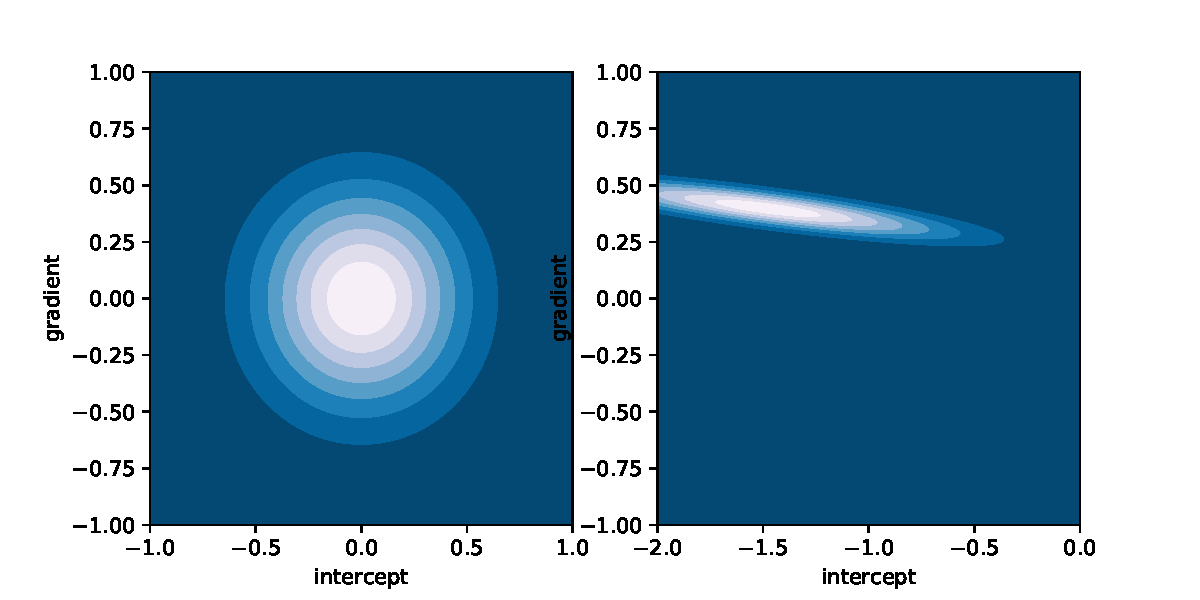
\includegraphics[width=0.7\textwidth]{bayesregress.pdf}
\end{center}
\caption{Prior and posterior weight distribution after applying Bayesian regression on ten points.}
\label{fig-post}
\end{figure}



\begin{figure}[!ht]
\begin{center}
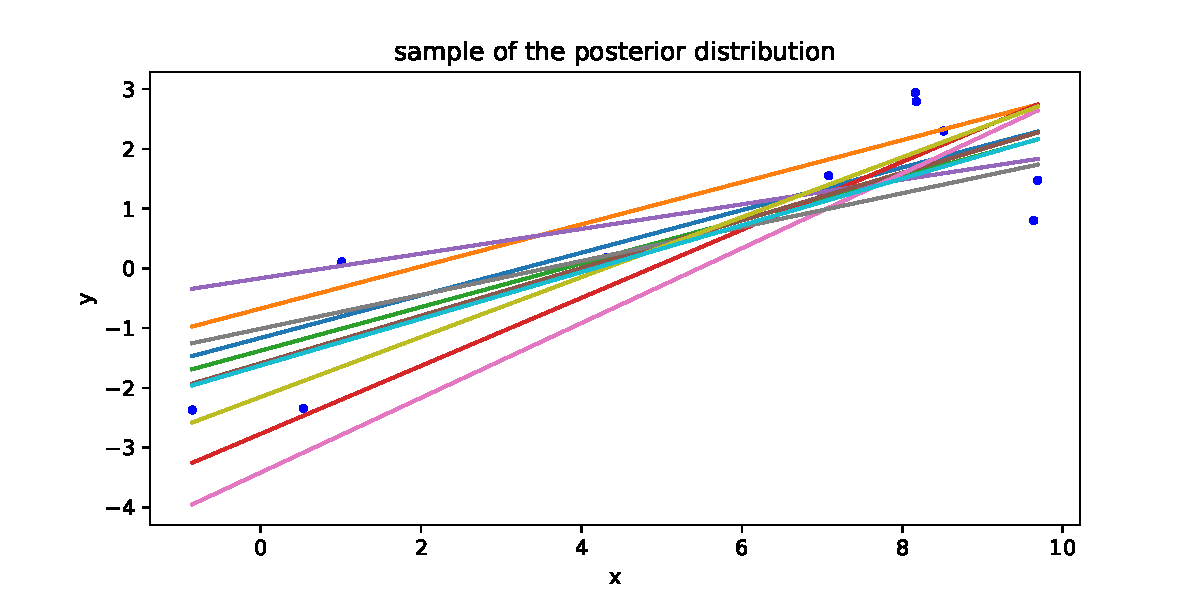
\includegraphics[width=0.7\textwidth]{postsample.pdf}
\caption{This plot shows 10 linear relationships that have been sampled from the posterior distribution, which was obtained by regressing on 10 data points.}
\end{center}
\end{figure}



\section{Pros and cons of Bayesian Regression}

\subsection{Predictive Distribution and Maximum a Posteriori}
Using the MLE of the weights is simple. Once the optimal weights have been obtained, the are inserted in the polynomial. Using the regression results for prediction is as simple as inserting a new $x$ value in the polynomial and obtain the corresponding $y$ value, which is the prediction for this $x$.

To properly use the posterior distribution of weights, one would have to calculate the weighted expectation with respect to the posterior distribution values over all weights:
$$
t = \int p(w \mid \boldsymbol{X}, \boldsymbol{t}) \boldsymbol{w}^T \boldsymbol{\phi}(x) dw
$$
A simple estimate would probably be to generate a number of samples of the posterior distribution as we've done above, where we sampled 10 linear relationships. We can than average the predictions made by each of these lines as an estimated of the *predictive distribution*.

In many cases this is huge overkill. If the idea is to use regression to get an approximate prediction, it is not necessary to use the posterior distribution. Sometimes a good compromise can be to use its maximum. In this particular case this would be given by the value of $\boldsymbol{m}_N$.  This is called the *maximum a posteriori* or *MAP*. Often a reasonable compromise, using the MAP is not entirely without risks, see for example section 5.2.1.2 of Murphy (2012).

In other cases, where little data is available and the penalty on a wrong decision based on MLE is severe it is better to accept the extra cost of the predictive distribution. In Unit 4 we will consider the case of determining whether a given point is an outlier. Such a decision may have financial or even legal consequences and here the importance of a principled estimate may outweigh the cost associated with evaluating the predictive distribution.


\subsection{Regularisation}

Bayesian models are far less prone to overfitting than MLE estimates, when applied consistently. The discussion for why this is the case becomes rather technical, but when two models explain the data adequately, the Bayesian approach favours the model with a smaller number of parameters.  This important aspect of Bayesian models is discussed in Section 3.4 and 3.5 of Bishop, but requires that you have digested most of the material earlier in Chapter 3 which goes into greater detail than we can do here.

We have seen that the Bayesian approach gives a posterior distribution of weights:
$$
p(\boldsymbol{w} \mid \boldsymbol{t} ) = \mathcal{N} ( \boldsymbol{w} \mid \boldsymbol{m}_N, \boldsymbol{S}_N),
$$
where you have derived the formulae for $\boldsymbol{m}_{N}, \boldsymbol{S}_N$. You should be able to verify that:
$$
\ln p(\boldsymbol{w} \mid \boldsymbol{t} ) = -\frac{\beta}{2} \sum^N_{i=1} \left\{ t_i - \boldsymbol{w}^T\boldsymbol{\phi}(x_i) \right\}^2  - \frac{\alpha}{2} \boldsymbol{w}^T \boldsymbol{w} + \mbox{const}
$$ 

Maximising the likelihood is equivalent to maximising the log likelihood, which in turn is equivalent to minimising
the quantity:
$$
L = \sum^N_{i=1} \left\{ t_i - \boldsymbol{w}^T\boldsymbol{\phi}(x_i) \right\}^2  + \frac{\alpha}{2\beta} \boldsymbol{w}^T \boldsymbol{w} 
$$
The first term is a sum of squares, which also emerges in least squares. The second term effectively is a penalty term for large weights. This is called a *regularisation* term, as it puts constraints on the magnitude of the weights. A perfect fit which reduces the first term can still be spoilt if the weights to achieve it attain large values and in the earlier examples we saw this exactly what happens when we overfit a simple dataset.

$L$ is sometimes called a \emph{loss function} (for training purposes - not to be confused with a prediction loss, see the discussion in Section 1.5.5. of Bishop (2006)). Minimising it can be seen as an optimisation problem. In this unit we have achieved minimisation by analytic means, but in the following units we will often see loss functions that we have to minimise using numerical methods.

Modern neural network frameworks often allow the definition of models and an independent specification of loss
functions. The *mean squared error* is a choice that is often made:
$$
\mbox{MSE} = \frac{1}{N}\sum^N_{i=1}(y_i - t_i)^2,
$$
and given the discussion so far it is not hard to see why it is an obvious choice, although it is by no means the only  and often not the best one. Statisticians use a slightly different definition that incorporates the number of parameters.

Neural network frameworks also often the possibility for different forms of regularisation. The research into Bayesian neural networks is in its infancy (see \cite{jospin2020} for a recent review), but regularisation offers some protection to overfitting.


\chapter{Information Theory and Probability}
\section{Introduction}
In machine learning it is important to establish whether or not events are distributed as expected. If not, we cannot make accurate predictions about new events. We may have to
adapt the distributions that we are comparing our events against, often by tweaking parameters, a process we call \emph{learning}. The requires that we develop a quantitative
measure to what extent past events conform to a given distribution. An interesting approach to this problem comes from information theory.

The key ideas are simple. Imagine that we have events that we measure at some remote station, which may fall in four categories: 'a', 'b', 'c' and 'd'. To transmit the occurances
of each event we may use four bits: we can transmit the combinations '00', '01', '10', '11' and use a code book linking these messages to the four categories. Assuming that
all occurrences are equally likely, this is the best we can do. If there were not four but sixteen categories, we would need 4 bits: '0000', etc. Binary words can use
$2^N$ combinations using $N$ bits. If all combinations are equally likely, it therefore makes sense to measure the information in terms of the number of bits required
to transmit an event $x$:
$$
h(x) = -^2\log p(x).
$$

Here $p(x)$ is the probability of the event which is the inverse of the number of possibilities, and therefore a minus sign is necessary to get a positive number of bits.
When the probability for different categories is not uniform, it makes sense to adapt the coding scheme.  In the example of 8 events $\{a, b, c, d, e,f, g, h\}$,
with probabilities $(\frac{1}{2}, \frac{1}{4}, \frac{1}{8}, \frac{1}{16}, \frac{1}{64}, \frac{1}{64}, \frac{1}{64}, \frac{1}{64} )$, it make sense to use
a more efficient code \cite{cover1999} (as presented in \cite{bishop2006}). If we were to ignore the difference in probabilities, we would have to assign 3 bits to each category
to transmit an event. But if we use the following code strings 0, 10, 110, 1110, 111100, 111101, 111110, 111111, then on average we will transmit less bits.

This difference can be quantified using \emph{entropy}: given a probability distribution $p(x)$ it is given by:
\begin{equation}
  \mathbb{H}[x] = - \sum p(x) ^2\log p(x)
\end{equation}
Note that this can be interpreted as the information averaged over all probabilities in the two examples we have given here. If we  assign uniform probability to
each of the 8 outcomes, we find:
$$
\mathbb{H}[x] = - 8 \times \frac{1}{8} ^2 \log \frac{1}{8} = 3,
$$
i.e. 3 bits.

If we calculate the average coding length under the probabilities listed above, using the coding scheme given above we find that it is:
$$
\frac{1}{2} \times 1 + \frac{1}{4} \times 2 + \frac{1}{8} \times 3 + \frac{1}{16} \times 4 + 4 \times \frac{1}{64} \times 6 = 2,
$$
so 2 bits.
If we work out $\mathbb{H}[x]$ for that probability distribution, we also find 2 \emph{by the same calculation}.
This suggests an interpretation of $\mathbb{H}$ as average code length.
The unequal distribution of probabilities allows a slightly more efficient transmission than the three bits per event that we found for equal probabilities. This idea
is reminiscent of Morse code, which uses a short set of dashes and dots for letters that occur often (the 'e' is a '.'). 
You may wonder about why the particular code was chosen. This code allows the concatenation of events in longer strings, but allows an unambiguous resolution into
individual event strings. You should check this.

The use of $^2 \log$, logarithms with base 2 is relatively uncommon, and the natural logarithm is often preferred. If we write:
$$
\mathbb{H}[x] = -\sum  p(x) \ln p(x),
$$ 
this amount to a change in units as changing the base of a logarithm multiplies the previous outcome by a constant factor. When we apply the natural logarithm, we no longer
measure entropy in bits, but in nats.

Further credence to the interpretation of entropy as a measure of the average content carried by an event can be lent by the following observations:
\begin{itemize}
\item  If only a single outcome has probably one, and all other potential possible outcomes have probability 0 then
  $\mathbb{H} = 0$. This requires an interpretation of $0 \ln 0$ as 0, which is justified since $\lim_{\epsilon \rightarrow 0} \epsilon \log \epsilon = $.
\item The entropy for a given set of outcomes is maximal if all outcomes are equiprobable. 
\end{itemize}
The analogy  between entropy and the amount of information that can be transmitted holds only strictly
for probability distributions which can be expressed as powers of $\frac{1}{2}$. For arbitrary
distributions  the entropy is a lower bound of the the information that can be transmitted using the best possible code. This is the essence of the \emph{noiseless
  coding theorem} which is due to Shannon \cite{bishop2006}. We will nonetheless stick to the code book metaphor as it provides good intuition for some of the
measures that we will introduce below.


Note that it is possible to express the amount of information associated with a certain event in terms of the probability of its outcome, again this $p_i \ln p_i$, where
$p_i$ is the probability of outcome $i$. This can be interpreted as the amount of nats required to store or transmit the event if an optimal code were to be used.
The central role played by the logarithm in information theory is explained by the property of logarithms in any base:
$$
\log(ab) = \log(a) + \log(b)
$$
It is the only function with this property. It states that when possibilities multiply, information content adds. This should be clear from the examples above and you
should now have an intuition for why logarithms play a central role in quantifying amounts of information.



The notion of entropy can be extended to continuous distributions but a subtlety occurs. Assume that the interval on which a continuous distribution is defined
is split into a finite number of bins, each of width $\Delta$. 
Assuming $p(x)$ is continuous, there exists an $x_i$ such that
$$
\int^{(i+1)\Delta}_{i\Delta} p(x) dx = p(x_i) dx 
$$
So, for a given discretisation the entropy can be written as:
$$
\mathbb{H}_{\Delta} = - \sum_i p(x_i) \Delta \ln(p(x_i) \Delta) = \sum_i \Delta \ln p(x_i) - \ln \Delta
$$
We omit the second term and then consider the limit $\Delta \rightarrow 0$. The first term on the righthand side then converges to
$$
\lim_{\Delta \rightarrow 0} \sum_i p(x_i) \Delta \ln p(x_i) = - \int p(x) \ln p(x) dx
$$
The integral is called \emph{differential entropy}. It differs from the entropy by a term $\ln \Delta$ which diverges when $\Delta$ converges to 0. This
reflects the fact that in a continuous distribution an infinite number of bits is required to register an event with total precision. In practice we are
typically limited by machine precision and $\ln \Delta$ would be finite, but since it would be a constant contribution to every entropy formulation we are
not particularly interested and simply omit in from our considerations.

For a multivariate density $p(\boldsymbol{x})$ the differential entropy is given by:
$$
\mathbb{H}[\boldsymbol{x}] = \int p(\boldsymbol{x}) \ln p(\boldsymbol{x}) d \boldsymbol{x}
$$


The following relationship sometimes appears in the literature, so we give it for completeness:
Given a joint distribution $p(\boldsymbol{x}, \boldsymbol{y})$, assume that pairs of $\boldsymbol{x}, \boldsymbol{y}$ are drawn. Assume that
the values of $\boldsymbol{x}$ is already known. The additional information needed to specify the corresponding value $\boldsymbol{y}$ is then
$-\ln p(\boldsymbol{y} \mid \boldsymbol{x})$. The average information needed to specify $\boldsymbol{y}$ can be written as:
$$
\mathbb{H}[\boldsymbol{y} \mid \boldsymbol{x}] = - \int \int p(\boldsymbol{y}, \boldsymbol{x}) \ln p(\boldsymbol{y} \mid \boldsymbol{x}) d \boldsymbol{y} d \boldsymbol{x}
$$
using the product rule, this reads as:
$$
\mathbb{H}[\boldsymbol{x}, \boldsymbol{y} ] = \mathbb{H}[ \boldsymbol{y} \mid \boldsymbol{x} ] + \mathbb{H}[\boldsymbol{x}]
$$
Here $\mathbb{H}[\boldsymbol{x}, \boldsymbol{y}]$ is the differential entropy of $p(\boldsymbol{x}, \boldsymbol{y})$ and $\mathbb{H}[\boldsymbol{x}]$ is the
entropy of the marginal distribution $\mathbb{H}[\boldsymbol{x}]$. So the information required to specify $\boldsymbol{y}$ is the information required to
specify $\boldsymbol{x}$ together with the extra information to specify $\boldsymbol{y}$ given $\boldsymbol{x}$.
\section{Relative Entropy}
Above, we introduced the notion of a code where the number of bits used to represent an event is coded is inversely proportional to  the logarithm of the probability of
the outcome of that event. That presupposes that we actually know this probability distribution. What if we have designed a code based on a probability distribution $p(x)$,
when the actual distribution is a different one $q(x)$. We would be able to tell, because as we would collect events and store them on disk,
we would need more information to record them than we would have expected. 

Assume we want to transmit events based on a probability distribution  $p(x)$. If we were to use a code book based on probability distribution $q(x)$,
we will find that in general we will need to store a larger amount of information than if we had used a code book based on the true distribution $p(x)$.
The amount of extra information is:
\begin{align}
  \mbox{KL}(p \mid \mid q) &  = - \int p(x) \ln q(x) df - (- \int p(x) \ln p(x) dx ) \nonumber \\
                           &  = - \int p(x) \ln \{ \frac{q(x)}{p(x)} dx
\end{align}

This is the \emph{Kullback-Leibler} or \emph{KL-divergence}, sometimes also called \emph{relative entropy}. We will show that
$$
\mbox{KL}(p \mid \mid q) \ge 0
$$
and that only when $p(x) = q(x)$ for all $x$ , $\mbox{KL}(p \mid \mid q) = 0$. This underpins the statements made above that when using the 'wrong' code book, messages
will be longer than they need to be.

All this implies that the KL-divergence can be used as a measure for how far two distributions diverge. It is not called a metric because it is asymmetric in its arguments, i.e.
in general
$$
\mbox{KL}(p \mid \mid q) \ne \mbox{KL}(q \mid \mid p).
$$
As we will see, it derives its usefulness in part from this property.

\begin{figure}
\begin{center}
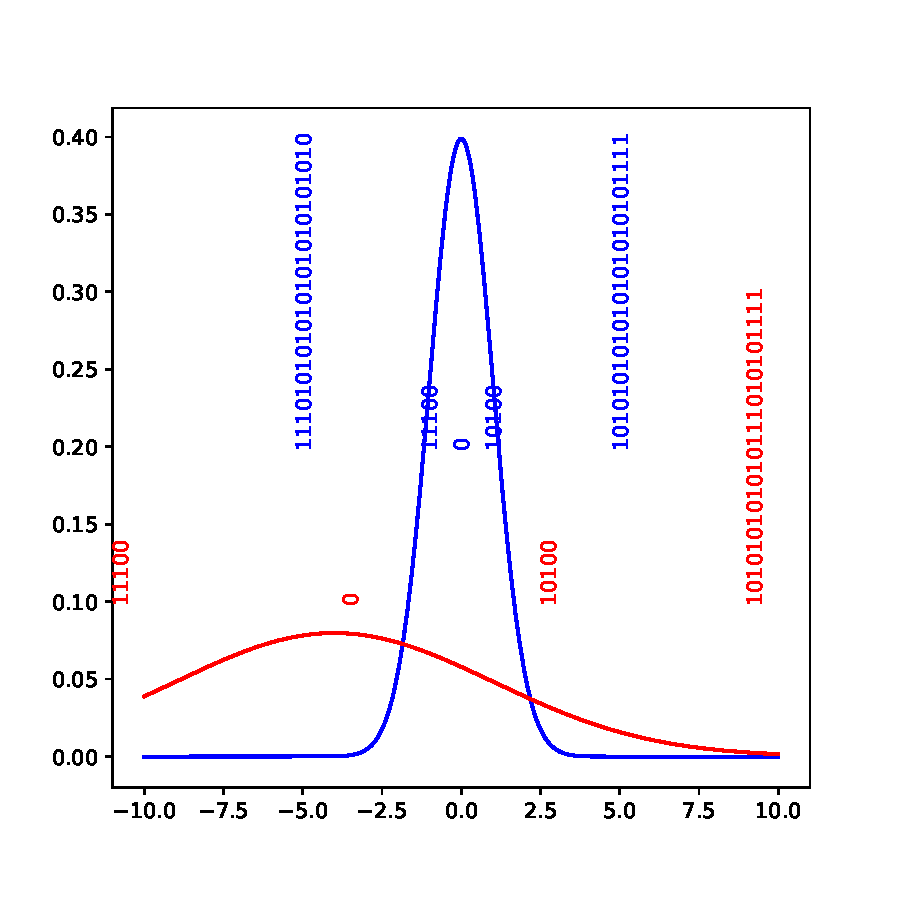
\includegraphics[width=0.7\textwidth]{kl.pdf}
\end{center}
\caption{Events can be coded by a code book tailored to the red distribution or the blue distribution. When events are distributed according to the red distribution, they are more efficiently coded by the 'red' code book. Most events of the red distribution would fall well outside regular events according to the blue distribution, so using the 'blue' code book would lead to a huge increase in message size. The opposite is also true: events generated by the blue distribution are more efficiently code by the 'blue' code book, but events generated by the blue distribution could have plausibly come from the red distribution. This would lead to a longer message size if the 'red' code book were used although not nearly as much as in the opposite case. The KL-divergence is asymmetric in its arguments.}
\label{fig-kl}
\end{figure}

Consider Fig. \ref{fig-kl}. There is a blue and a red distribution. If events are distributed according to the blue distribution, their values are likely to be close
to the peak of the blue distribution. A 'blue' code book would assign shorter bit sequences to those events, and longer ones to events well away from the peak because
they are rare. Similarly for the red distribution. If we were to use the 'red' code book for events distributed according to the blue distribution, we would incur a penalty
in terms of message length, because these events are somewhat away from the red centre and therefore would be longer sequences. Using the 'blue' code book
for red events would be horrendous: most events of the red distribution cannot be plausibly generated by the red blue distribution. Only when the right code book
is used for the right distribution of events is the message length minimal.

A real example in statistics would be to assume a Gaussian for events that are distributed according to a student distribution. The latter would be likely to generate
outliers in a relatively small sample that could not have been plausibly generated by a Gaussian. It is this property that makes the KL-divergence an efficient
measure for divergence between two probability distributions.

Now suppose we sample data from an unknown distribution $p(x)$, which we may want to represent by a known distribution $q( \mid \theta)$ , where $\theta$
are adjustable parameters. It would be nice to estimate the KL-divergence but the true distribution $p(x)$ is not available. If we have a finite set
of data $x_i$, $i = 1 \cdots M$ drawn from distribution $p(x)$ we can approximate the KL-divergence by

$$
\mbox{KL}( p \mid \mid q) \approx \sum^N_{i=1} \left\{ -\ln q(x_n \mid \theta) + \ln p(x_n) \right\}.
$$
The second term is independent of $\theta$ so minimising the KL-divergence with respect to $\theta$ is equivalent to maximising the likelihood function. In Unit 2, we will
see how loss functions can be motivated based on the KL-divergence because of this.
    
\section{Jensen's Inequality}
The use of the KL-divergence as a measure that quantifies the inequality of two probability functions as a positive number rests on a simple mathematical theorem
called \emph{Jensen's inequality}. You will not be assessed on deriving it, but it occurs in many places in the machine learning literature. Alternatives exist to using
the KL-divergence, e.g. \emph{free energy}, but this too relies on Jensen's inequality. It is worth knowing about and being able to look up its proof when you encounter
it in the literature.

\begin{figure}[!ht]
\begin{center}
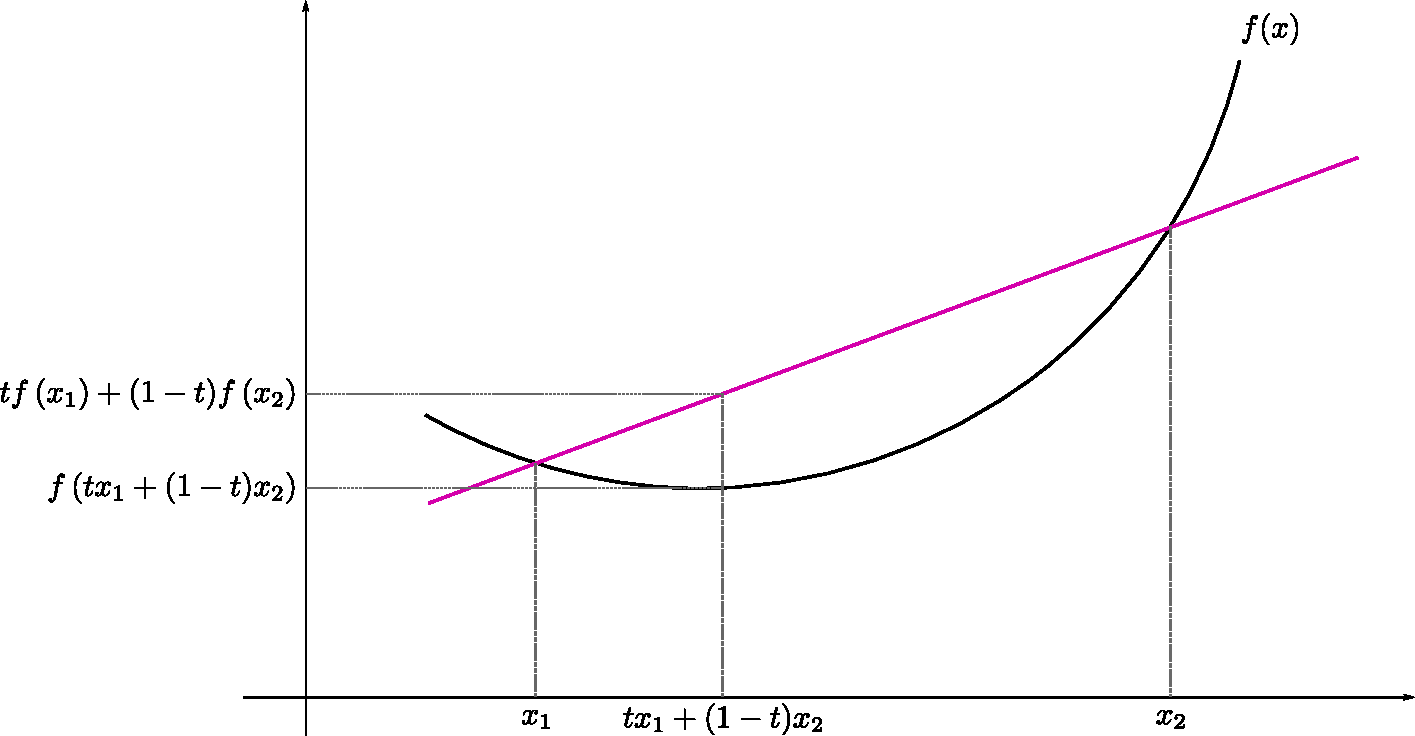
\includegraphics[width=0.7\textwidth]{ConvexFunction.pdf}
\end{center}
\caption{Jensen's inequality as a cord above a convex function. Source: Wikimedia.}
\label{fig-convex}
\end{figure}

A convex function is a function whose second derivative is positive everywhere. Examples are $f(x) = x^2$ and $g(x) = x \ln x$. An example is shown in Fig. \ref{fig-convex}.
Consider a point of the purple line between $x_1$ and $x_2$. It is intuitively obvious that the entire purple line lies above $f(x)$ when $x_1 < x < x_2$. More precisely,
$$
tf(x_1) + (1-t)f(x_2) \ge f(t x_1 + (1 - t) x_2),
$$
with strict inequality for $x_1 < t < x_2$ is $f(x)$ is strictly convex in that interval.

This is Jensen's inequality.

Using induction, this inequality can be proven for higher dimensions as well \cite{bishop2006} (exercise 1.38) and then reads:
\begin{equation}
  f(\sum^M_{i=1} \lambda_i x_i) \le \sum^M_{i=1} \lambda_i f(x_i),
 \end{equation}
where $\lambda_i \ge 0$ and $\sum_i \lambda_i =1$.
By taking the values $x_i$ as a discrete set, we can interpret the $\lambda_i$ as a probability distribution over the discrete variables $\{ x_i \}$. In that
case Jensen's inequality can be written as:
$$
f(\mathbb{E}[x]) \le \mathbb{E}[f(x)].
$$
There is a nice graphical interpretation of this inequality that can be found on Wikipedia:
\begin{figure}[!h]
  \begin{center}
    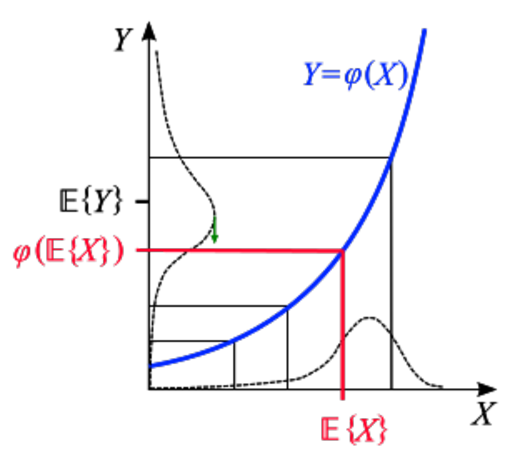
\includegraphics[width=0.8\textwidth]{Jensen_graph.pdf}
  \end{center}
  \caption{A graphical interpretation for $f(\mathbb{E}[x]) \le \mathbb{E}[f(x)]$.
 Source: Wikipedia.}
  \label{fig-jensen}
\end{figure}
Consider Fig. \ref{fig-jensen}. An arbitrary probability distribution can be found in the bottom of the plot with the density displayed as a function
of $X$. The expectation value $\mathbb{E}[X]$ is shown in red and is slightly to the left of the bulge, due to the heavy tail extending to the left.
A convex function $\phi(x)$ is the applied to all $x$ values. The variables $y$  are shown on the vertical axis. An interval in $x$, will be transformed
into an interval in $y$ and this interval in $y$ must contain the same fraction of events as the interval in $x$. This leads to a transformation
of the probability density over $X$ into one over $Y$. It is clearly visible  that the distribution is more stretched towards the higher the values in $y$.
So you can look at the transformed value of the expectation value, $\phi(\mathbb{E}[X])$ and compare it to the expectation value $\mathbb{E}[y]$, the
expectation value of the $y$-distribution. The latter is always higher because the convex function $\phi(x)$ stretches larger values of $x$ more than smaller values. This is
the geometrical intuition underlying Jensen's inequality.

A final point that is both trivial and subtle. We can rewrite Jensen's inequality because the actual values of the $x_i$ are immaterial. Suppose there is a function
$y=g(x)$. Jensen's inequality only cares about the convexity of the function $f(x)$, not the value of the $x_i$. So written in terms of $y_i$, it is still true that:

$$
  f(\sum^M_{i=1} \lambda_i y_i) \le \sum^M_{i=1} \lambda_i f(y_i),
  $$

In other words, Jensen's inequality can also be written as:
$$
  f(\sum^M_{i=1} \lambda_i g(x_i)) \le \sum^M_{i=1} \lambda_i f(g(x_i)).
  $$
  



  
For continuous variables, this becomes:
\begin{equation}
  f( \int \boldsymbol{x} p(g(\boldsymbol{x})) dx ) \le \int f(\boldsymbol{x}) p(g(\boldsymbol{x})) d \boldsymbol{x}
\end{equation}



\begin{figure}
  \begin{center}
  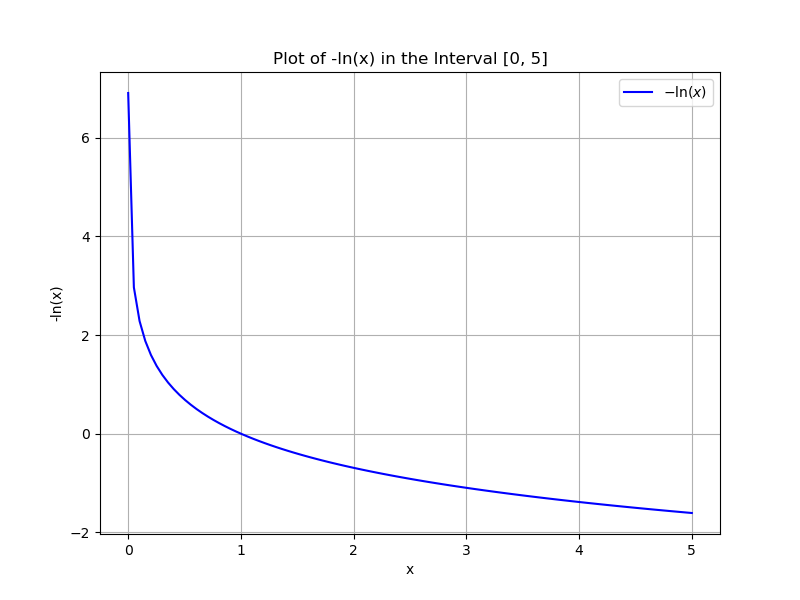
\includegraphics[width=0.8\textwidth]{log.png}
  \end{center}
  \caption{$ -\ln x$ is a convex function.}
  \label{fig-log}
\end{figure}

Now we can apply this inequality to the KL-divergence. So far, we have discussed Jensen's inequality in terms of an abstract convex function. One such function is:
\begin{equation}
  f(x) = -\ln x
\end{equation}
Remember that this function plays a central role in this story due to its appearance in the entropy definitions. For completeness, we show a plot of
$f(x) = -\ln x$ in Fig \ref{fig-log}. We can now use the definitions:
$$
f(x) = -\ln x
$$
and
$$
g(x) = \frac{q(x)}{p(x)}
$$.


\begin{equation}
\mbox{KL}(p \mid \mid q) = - \int p(\boldsymbol{x}) \ln  \left\{ \frac{q(\boldsymbol{x})}{p(\boldsymbol{x})}
\right\}  d \boldsymbol{x} \ge -\ln \int q( \boldsymbol{x}) d \boldsymbol{x}
\label{eq-kl}
\end{equation}
Here we used that $\int q(\boldsymbol{x}) d \boldsymbol{x} = 1$, as $q(\boldsymbol{x})$ is a probability distribution and the fact that $-\ln x$ is a strictly
convex function, so that equality will only hold when $p(\boldsymbol{x})= q(\boldsymbol{x})$.

This proof is important as it confirms what we so far based on intuition: using the 'wrong' probability distribution to define a code book
\emph{always} leads to longer messages. Moreover, the properties of the KL-divergence are not really dependent on our intuition any more.
Although it is useful to think of entropy and KL-divergence in terms of information theory, Eq. \ref{eq-kl} shows that the properties
of the KL-divergence are based on Jensen's inequality and as such can be rigorously defined, independent of a coding length metaphor.


\chapter{Some Cautions}
The material presented here is intended to provide the theoretical framework
for the later material. It is not suitable for the analysis of real world data without
further reading. We have not discussed the need for more robust inference
when data contains \emph{outliers}. At the very least, you should consult
section 7.4 of \cite{murphy2012}. In Unit 5 you may find useful techniques
to model outliers as a mixture of different processes.

From this unit you may have received the impression that Bayesian analysis is the
norm. It is not. Its use, in particular with complex models such neural networks
is in its infancy. The main problem is that a neat interpretation of the posterior
in terms of the parameters of a distribution is possible in only the simplest
of cases. Even in logistic regression (Unit 2), only a numerical
estimate of the posterior is possible and this is a huge complication in its
own right. Unit 4 and 5 deal with methods to alleviate this problem.


  
  


  


